\documentclass[]{homework}
\usepackage{calrsfs}
\usepackage[caption=false,font=footnotesize]{subfig}
\usepackage[section]{placeins}
\studname{Amal Alabdulkarim (aa4235), 
Danyang He (dh2914), Jing Qian (jq2282)}
\coursename{COMS 4771: Machine Learning (Fall 2018)}
\hwNo{4}
\begin{document}
\maketitle

%%%%%%%%%%%%%%%%%%%%%%%%%%%%%%%%%Problem 1%%%%%%%%%%%%%%%%%%%%%%%%%%%%%%%%%
\section*{Problem 1}
\subsection*{(a)}
The VC-dimension of the class the set F of binary classifiers induced by axis aligned rectangles in D dimensions is 2D. 
\begin{proof}
To proof the tightest possible bound on the VC-dimension we have to show an upper bound and a lower bound on the VC-dimension: 
\begin{enumerate}
    \item VC-dimension of $F \geq 2D$ \\ %lower bound
    Consider a set of points S and $|S| = 2D$, where we have every 2 points symmetrical around each dimension. So they would create an imaginary rectangle in the $D$ dimension, where every point is orthogonal to one surface of the rectangle and the number of points is equal to the faces of the rectangle. In this placement, every labeling of these points can be easily shattered by an axis aligned rectangle. Therefore, it the   VC-dimension of F $\geq 2D$.
    We can show this by an example in the 3 dimension in Fig.\ref{fig:rectangle1} and Fig.\ref{fig:rectangle2}. \\
    \begin{figure}[!h]
        \centering
        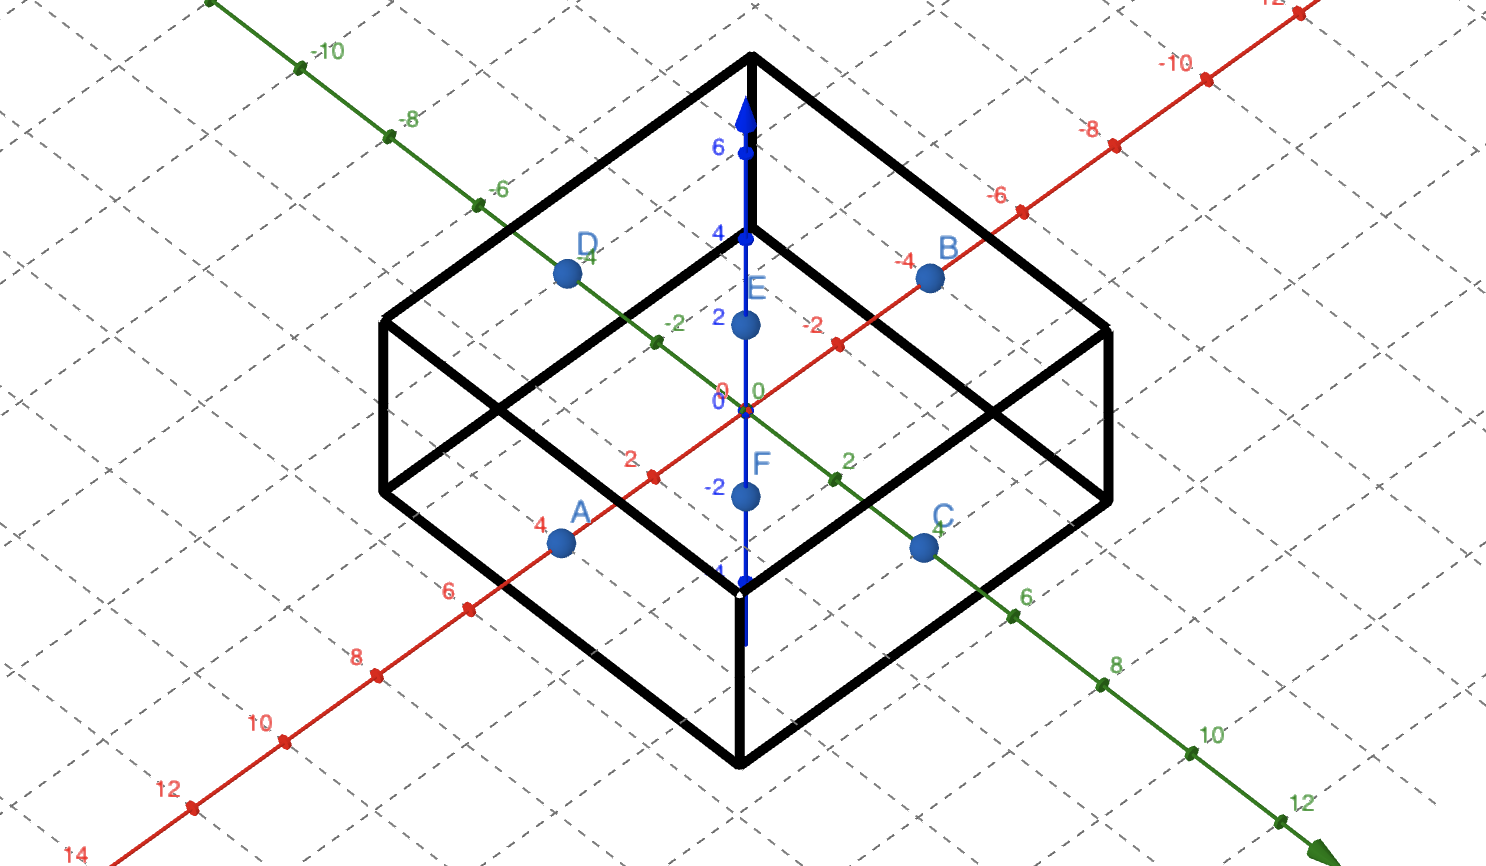
\includegraphics[width=4.5in]{figs/rectangle1.png}
        \caption{A positioning of 2D points in $D=3$, where all the points are on the surfaces of the rectangle have the same label (All negative).}
        \label{fig:rectangle1}
    \end{figure}
    If we change the labeling of each point we can shrink or extend the rectangle in that dimension to put the correct label on this point.
    \begin{figure}[!h]
        \centering
        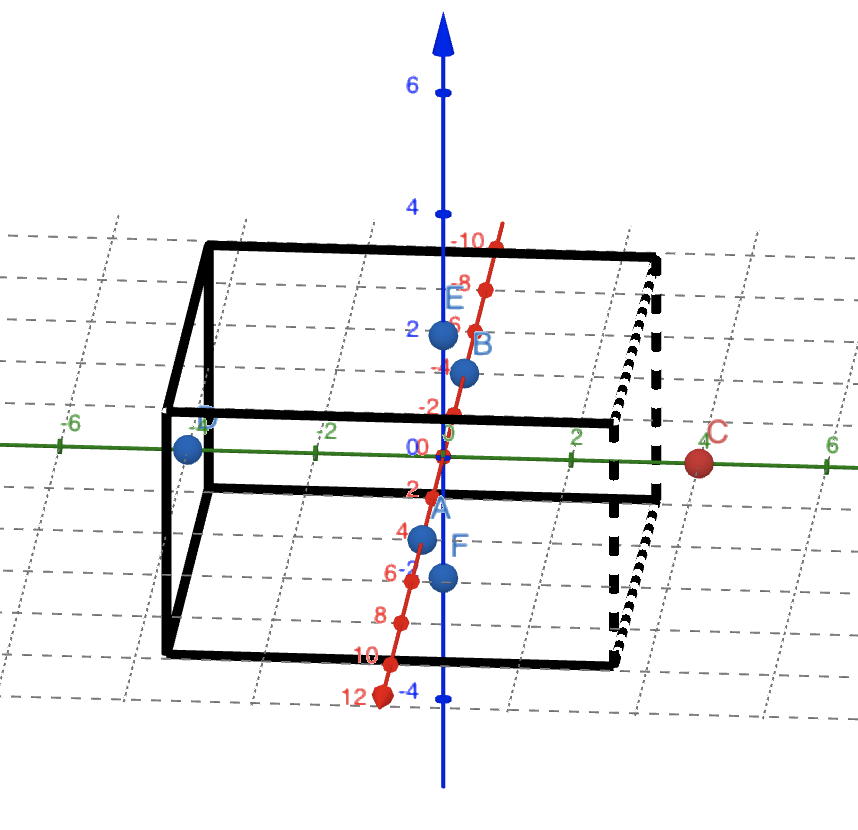
\includegraphics[width=4.5in]{figs/rectangle2.png}
        \caption{A positioning of 2D points in $D=3$, where all the points are on the surfaces of the rectangle after we changed the label of point C to positive.}
        \label{fig:rectangle2}
    \end{figure}
    
    \item  VC-dimension of F$ < 2D+1$
    
     %upper bound
    If the number of points is $2D+1$, then for any placement of $2D+1$ points, we can assign the point in the center of the other points to the  to +1, and all the other points to -1, which would make any set of $2D+1$ impossible to shatter by any rectangle in $D$.  
    
\end{enumerate}
    Now that we proved 1 and 2, this concludes the proof that the  VC-dimension of $F = 2D$. \\
\end{proof}
\subsection*{(b)} 
From the definition $G_1$ is the complement of $F$, then it is the class of all axis aligned rectangles in $D$ where the interior is labeled positive and the exterior is labeled negative. Therefore, it has the same VC-dimension of $F = 2D$. 
\subsection*{(c)} 
\begin{theorem}
H is efficiently PAC-learnable in the standard model, if and only if H is efficiently PAC-learnable in the two sample model.
\end{theorem}
\begin{proof}
To show this is true, we have to show that the two following claims hold. Only if both claims hold the theorem is valid.
\begin{claim}
If H is efficiently PAC-learnable in the standard one sample model then H is PAC-learnable in the two sample model
\end{claim}
\begin{proof}
Let us assume that we have algorithm A, which is a an algorithm for efficiently PAC-learning H in the standard one sample model given $\delta$ and $\epsilon$. It will output an $\varepsilon$-accurate hypothesis with probability $1-\delta$. 

We will show that we can use this algorithm in the two sample model and get a poly(n, $\frac{1}{\delta}$, $\frac{1}{\epsilon}$) time algorithm that has a polynomial sample complexity and outputs a $\varepsilon$-accurate hypothesis with probability $1-\delta$. 

Let's give A, $\delta$ and $\varepsilon$ and run it on the two sample model. 

To draw an example from the two sample model and given that both $D^+$ and $D^-$ follows the same distribution $D$, we will simulate the distribution $D$ using the two sample model by the use of a fair coin, we will toss the coin and if it comes head we draw en example from $D^+$ or we draw an example from $D^-$.

Because A has a $poly(n, \frac{1}{\varepsilon},\frac{1}{\delta})$ running time and drawing examples from the sample model takes O(1) time, then running it with this simulation will also be $poly(n, \frac{1}{\varepsilon},\frac{1}{\delta})$.

Now we calculate the error bounds to calculate the sample complexity: \\
The probability that A outputs a bad hypothesis $h_{A}$ that has error rate  $> \frac{\varepsilon}{2}$ on positive examples, given $err(h^*)=0$:
\begin{align*}
    Pr_+[err(h_{A}) - err(h^*) > \frac{\varepsilon}{2}] \leq exp(-2\frac{\varepsilon^2}{4}m) = exp(-\frac{\varepsilon^2}{2}m)
\end{align*}
The probability that A outputs a bad hypothesis $h_{A}$ that has error rate  $> \frac{\varepsilon}{2}$ on negative examples:
\begin{align*}
    Pr_-[err(h_{A}) - err(h^*) > \frac{\varepsilon}{2}] \leq exp(-2\frac{\varepsilon^2}{4}m) = exp(-\frac{\varepsilon^2}{2}m)
\end{align*}
The probability that A outputs a bad hypothesis $h_{A}$ that has error rate  $> \frac{\varepsilon}{2}$ on both positive and negative examples:
\begin{align*}
     &Pr[err(h_{A}) - err(h^*) > \varepsilon] = \\ &Pr_+[err(h_{A}) - err(h^*) > \frac{\varepsilon}{2}]+Pr_-[err(h_{A}) - err(h^*) >  \frac{\varepsilon}{2}] \leq 2exp(-\frac{\varepsilon^2}{2}m)
\end{align*}
We upper bound this error bound by $\frac{\delta}{|H|}$ and we use the union bound to account for all bad hypotheses and then we solve for $m$:
\begin{align*}
    |H|2exp(-\frac{\varepsilon^2}{2}m) &\leq \delta \\
    2exp(-\frac{\varepsilon^2}{2}m) &\leq  \frac{\delta}{|H|} \\
    exp(-\frac{\varepsilon^2}{2}m) &\leq \frac{\delta}{2|H|} \\
    \ln(exp(-\frac{\varepsilon^2}{2}m)) &\leq \ln(\frac{\delta}{2|H|}) \\
    -\frac{\varepsilon^2}{2}m &\leq \ln(\frac{\delta}{2|H|}) \\
    m &\geq \frac{2}{\varepsilon^2}\ln(\frac{2|H|}{\delta}) \\
\end{align*}

Which gives us an $\varepsilon$ accurate hypothesis with $1-\delta$ probability, with $m = poly(\frac{1}{\varepsilon^2},\frac{1}{\delta})$ sample complexity and polynomial running time. Which concludes the proof of the first claim, if H is PAC-learnable in the one sample model, then H is PAC-learnable in the two sample model.
\end{proof} 
\begin{claim}
If H is PAC-learnable in the two sample model then H is PAC-learnable in the standard one sample model
\end{claim}
\begin{proof}
Let us assume we have an algorithm B that is efficiently PAC-learning H in the two sample model given $\delta$ and $\varepsilon$ and it will output an $\varepsilon$-accurate hypothesis with probability $1-\delta$.

We will show that we can use this algorithm in the one sample model and get a poly($n, \frac{1}{\delta}, \frac{1}{\varepsilon}$) time algorithm that has a polynomial sample complexity and outputs a $\varepsilon$-accurate hypothesis with probability $1-\delta$. 

Let's give B, $\delta$ and $\varepsilon$ and run it in the one sample model.

To simulate a draw from the two sample model distribution, every time B requests an sample from $D+$ we will draw samples from $D$ until we get a positive sample and we return it to B. If we draw $m$ samples and found no positive samples we output all minus hypothesis $h^-$. And if we want to draw an example from $D-$ we draw from $D$ until we find a negative sample, if after $m$ samples we haven't found it, we output the all plus hypothesis $h^+$. Otherwise if we succeed every time in drawing the samples we output the hypothesis that B will output when given enough samples. 

The intuition behind this idea, is if the probability of finding a positive example is $\leq \varepsilon$ then if we output $h^-$ and make mistakes on all positive examples and make 0 mistakes on the negative, the hypothesis $h^-$ is still $\varepsilon$-accurate. Also, an analogous explanation is valid for the probability of finding a negative example if the output hypothesis was $h^+$.  So to make sure that this is valid, we need to find $m$ that is large enough to make sure that $h^-$, $h^+$, and all B output hypotheses will not make more than $\varepsilon$ mistakes with probability $1-\delta$.
\begin{align*}
    Pr[err(h_B) \geq \varepsilon] &= (1-\varepsilon)^m \\
                                  &\leq exp(-\varepsilon m) 
\end{align*}

We use the union bound over all hypotheses of B, and then we solve for $m$
\begin{align*}
     |H|exp(-\varepsilon m)  &\leq \delta \\
     exp(-\varepsilon m)  &\leq \frac{\delta}{|H|} \\
     -\varepsilon m  &\leq ln(\frac{\delta}{|H|}) \\
     m  &\geq \frac{1}{\varepsilon}ln(\frac{|H|}{\delta}) \\
\end{align*}
Which gives us an $\varepsilon$ accurate hypothesis with $1-\delta$ probability, with $m = poly(\frac{1}{\varepsilon},\frac{1}{\delta})$ sample complexity and polynomial running time. Which concludes the proof of the first claim, if H is PAC-learnable in the two sample model, then H is PAC-learnable in the one sample model. 
\end{proof}

By showing that claim 1 and claim 2 hold, we conclude the proof. 
\end{proof}

%%%%%%%%%%%%%%%%%%%%%%%%%%%%%%%%%Problem 2%%%%%%%%%%%%%%%%%%%%%%%%%%%%%%%%%
\section*{Problem 2}
\subsection*{(a)}
We can think intuitively that the possible minimum value of equation (1) is 0, with each data point in each cluster. Namely, $k$ = number of data points, and every $c_i$ = one data point $x_i$. So in this case, the algorithm does nothing. Every data point belongs to one distinct cluster and the cluster actually overfits to the dataset. If we receive a new datapoint, we would not know which cluster it belongs to.
\subsection*{(b)} 
\begin{figure*}[h!]
\label{figure1}
\centering
\subfloat[Original visualization]{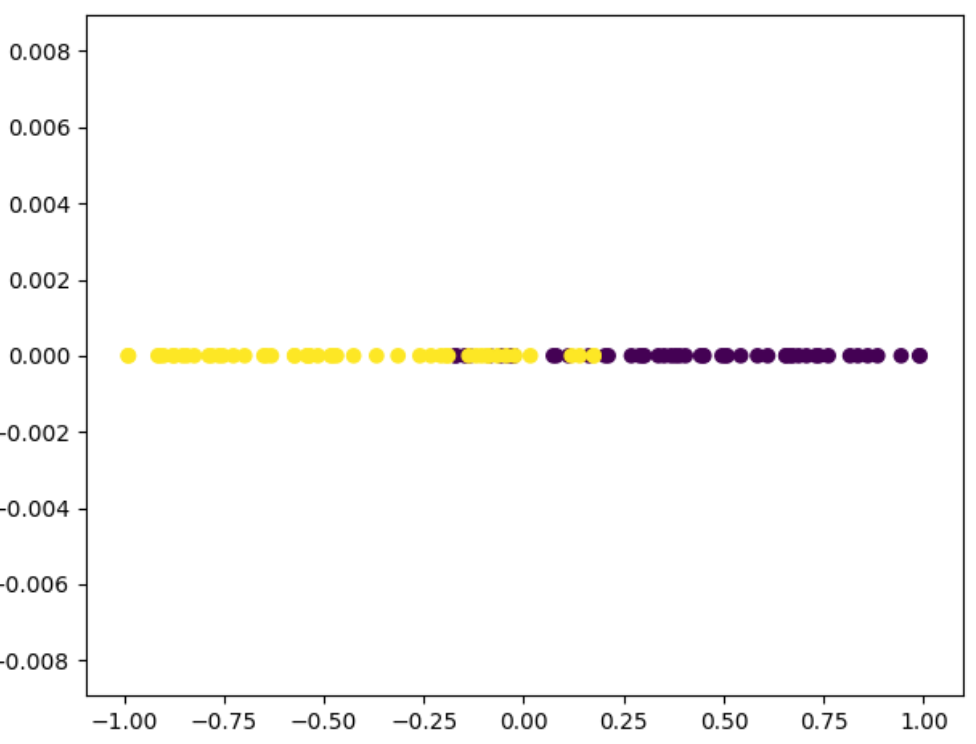
\includegraphics[width=2.5in]{figs/1d.png}}%
\label{figure2a}
\hfil
\subfloat[K-means visualization(blue and red points represent the two centroids respectively)]{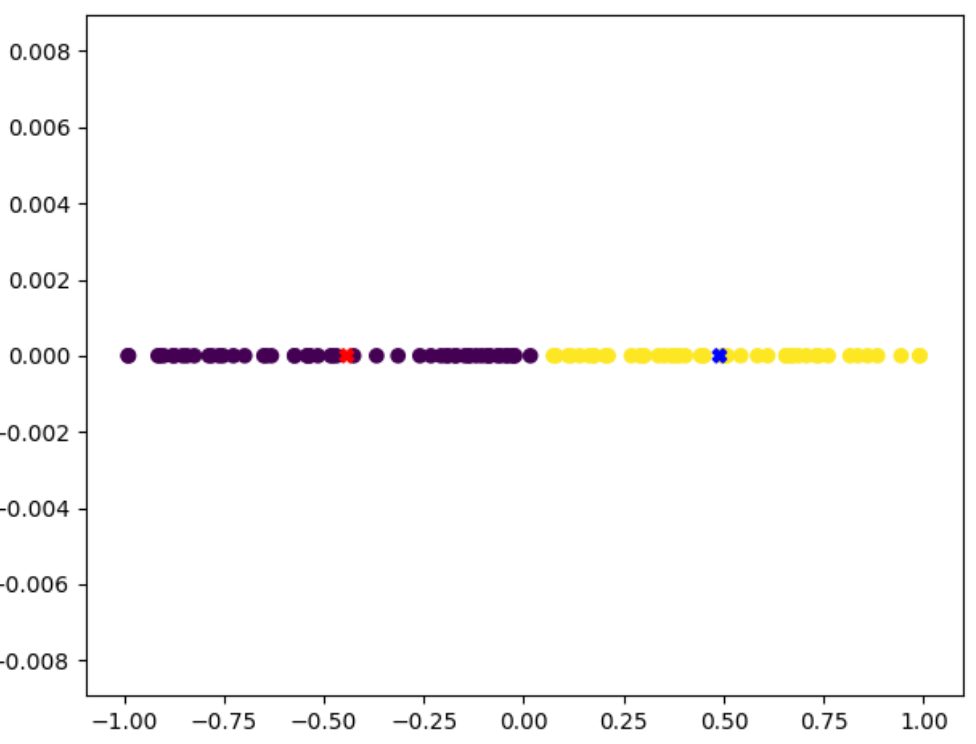
\includegraphics[width=2.5in]{figs/1dwrong.png}}%
\label{figure2b}
\caption{One dimensional datasets (a) original visualization and (b) k-means visualization}
\end{figure*}\par
As Figure 3 shows, when two clusters have overlap, the Lloyd's method will not achieve optimal setting. It will simply cut the data points into two clusters through the middle and that is because lloyd's method just uses L2 norm and only considers clustering data points that are close to each other in Euclidean distance.
\subsection*{(c)} 
\subsubsection*{(i)}
The Lloyd's method for K-means is based on two assumptions:
\begin{itemize}
    \item The clusters are spherical
    \item The variance of the clusters are in the same scale
\end{itemize}
This is easy to understand because Lloyd's method is based on L2 norm which is basically calculating the area composed of data centered around a centroid within a certain distance. Thus, we came up with two examples, each breaking one of the assumptions.
The first dataset example is data drawn from Gaussian Mixture model(size = 499), in which different clusters of Gaussian have different covariance matrix. The Lloyd's method K-means result turned out to be:
\begin{figure*}[h!]
\centering
\subfloat[Origial visualization]{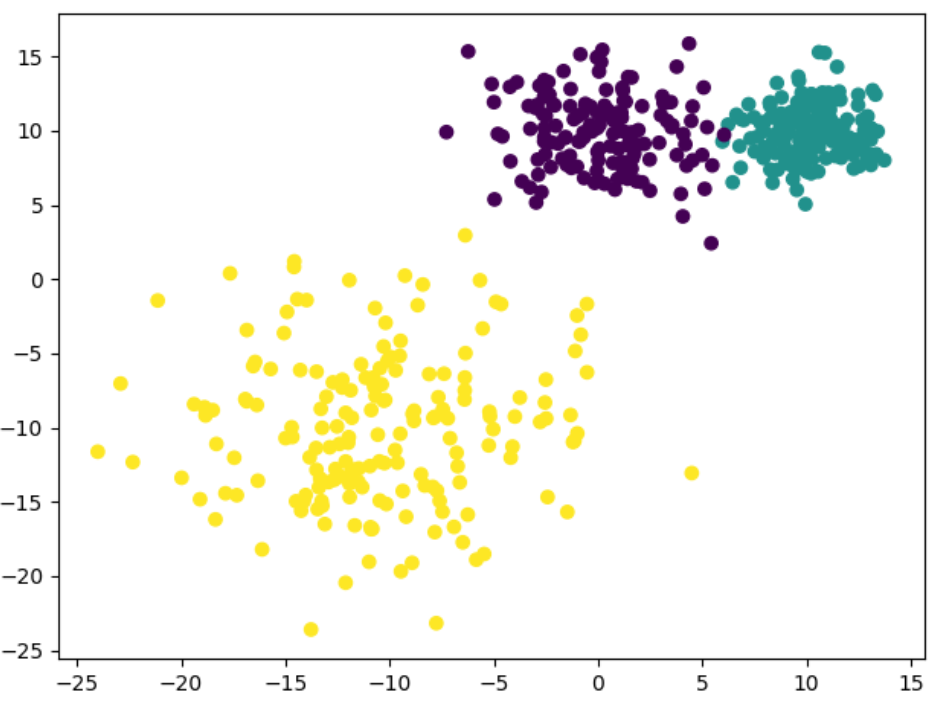
\includegraphics[width=2.5in]{figs/gmmoriginal.png}}%
\label{figure3a}
\hfil
\subfloat[K-means visualization]{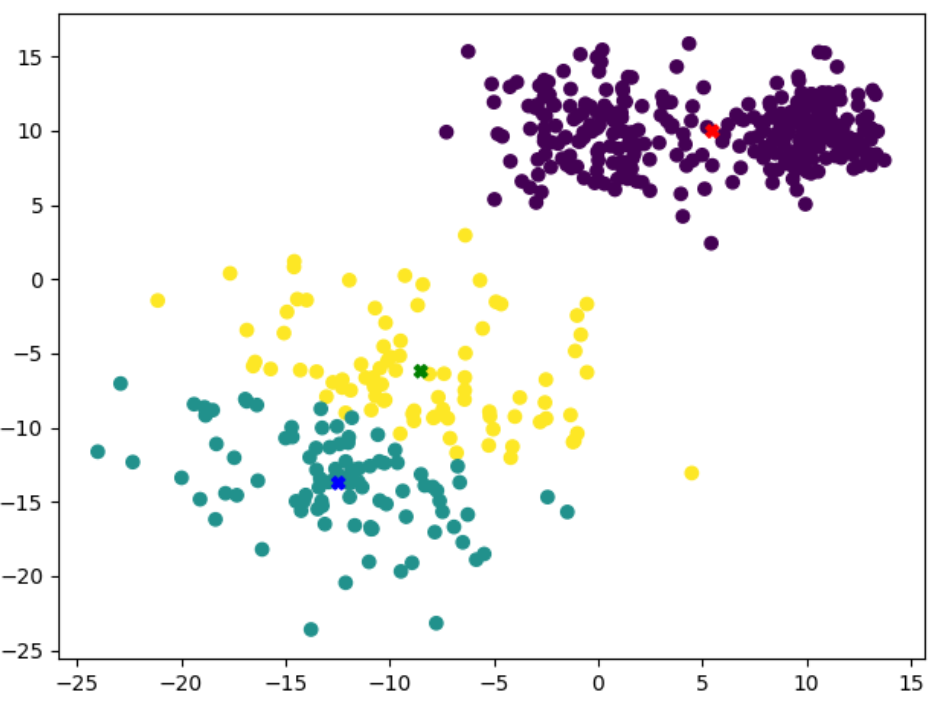
\includegraphics[width=2.5in]{figs/gmmkmeans.png}}%
\label{figure3b}
\caption{GMM datasets (a) original visualization and (b) k-means visualization. The three cluster has respective distributions: $purple \sim N(\begin{bmatrix}
   0\\ 10\\
  \end{bmatrix}, 3 I)$, $green \sim N(\begin{bmatrix}
   10\\ 10\\
  \end{bmatrix}, 6 I)$,$yellow \sim N(\begin{bmatrix}
   -10\\ -10\\
  \end{bmatrix}, 25 I)$
\end{figure*}\par
From the above two figures, we can see that when different clusters have different variance (not in same scale anymore), Lloyd's method fails and tends to split the bigger cluster and cluster the two smaller ones into one big cluster.
The other example we came up with is a non-linearly seperable dataset(size = 399):
\begin{figure*}[h!]
\centering
\subfloat[Origial visualization]{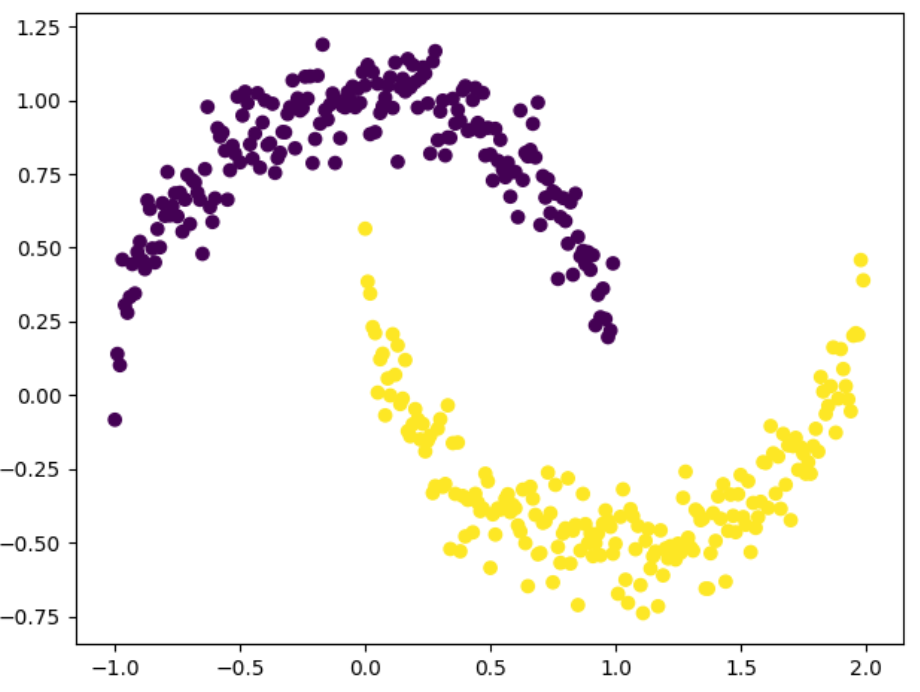
\includegraphics[width=2.5in]{figs/nonsphericaloriginal.png}}%
\label{figure2a}
\hfil
\subfloat[K-means visualization(blue points represent the centroids]{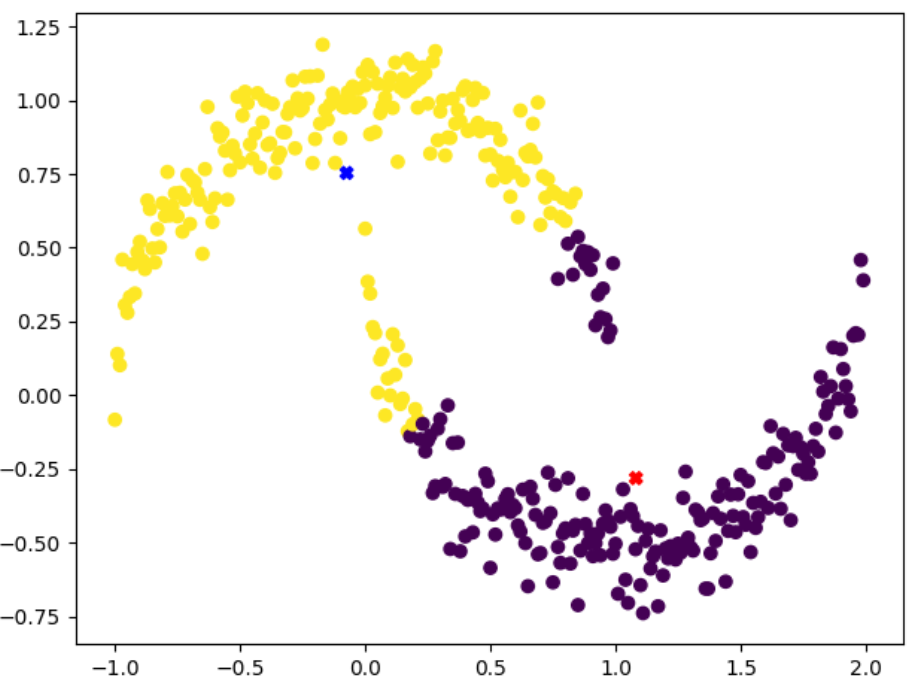
\includegraphics[width=2.5in]{figs/nonsphericalkmeans.png}}%
\label{figure2b}
\caption{Quadratic datasets (a) original visualization and (b) k-means visualization(The red and points represent two centroids respectively)}
\end{figure*}\par
from where we can see that Lloyd's method fails again because it tends to cluster datapoints that have the shortest Euclidean distance.
Besides, we came up with another dataset that is neither spherical nor in the same scale. The third example we came up with is a non-spherical spiral like dataset(size = 1149):
\begin{figure*}[h!]
\centering
\subfloat[Origial visualization]{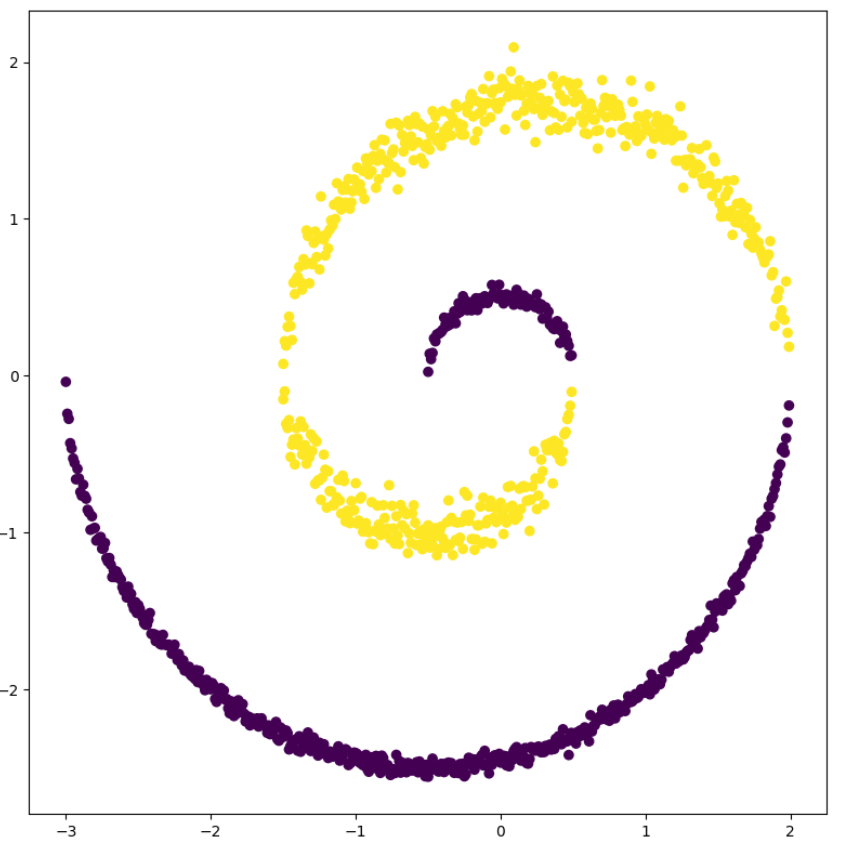
\includegraphics[width=2.5in]{figs/spiraloriginal.png}}%
\label{figure2a}
\hfil
\subfloat[K-means visualization(blue points represent the centroids]{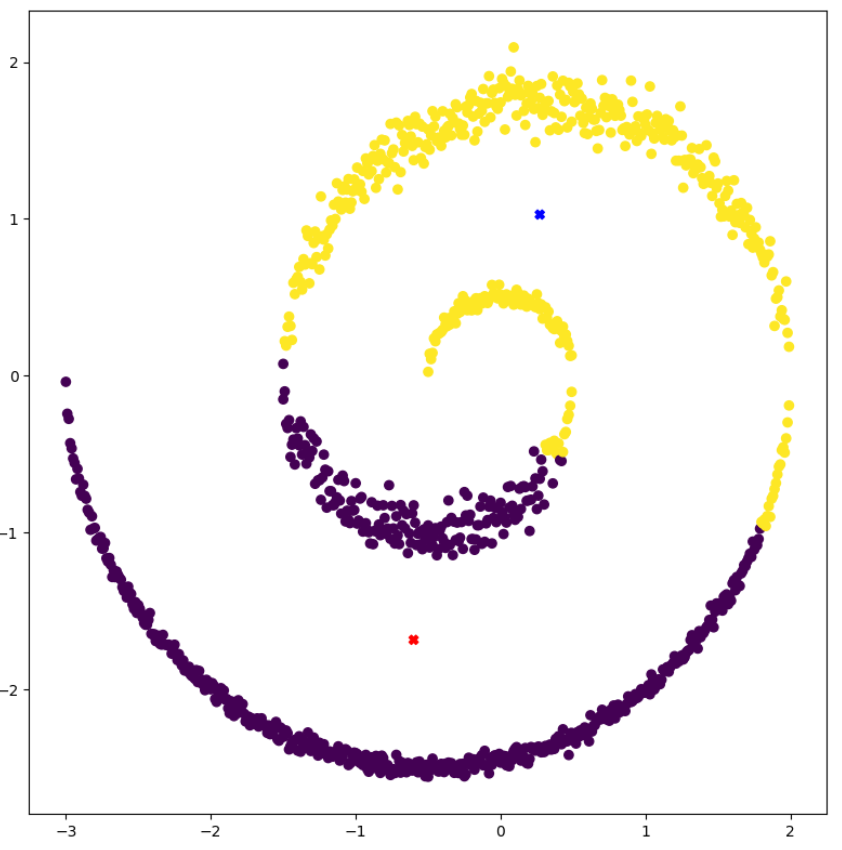
\includegraphics[width=2.5in]{figs/spiralkmeans.png}}%
\label{figure2b}
\caption{Spiral datasets (a) original visualization and (b) k-means visualization(The red and blue points represent two centroids)}
\end{figure*}\par
from where we can see that k-means fails as expected, clustering the data points that are close to each other into one cluster.
\subsubsection*{(ii)}
For $k = 2$ and any placement of $c_1$ and $c_2$, the cluster boundary will be linear because Lloyd's method uses L2 norm to select the minimum distance to cluster point to clusters. Thus, the cluster boundary should be the boundary on which data points have the same distance to each centroid. Thus, according to Bisection theorem\footnote{https://en.wikipedia.org/wiki/Bisection\#Line\_segment\_bisector}, the boundary should be the perpendicular bisector of the two centroids, and that yields a linear decision boundary.
\subsubsection*{(iii)}
To prove:
\begin{equation}
    \begin{aligned}
        f^T Lf &= \frac{1}{2} \sum_{ij} w_{ij} (f_i - f_j)^2
    \end{aligned}
\end{equation}
We do it from both the left hand side and the right hand side to make them equal to an intermediate value.
\begin{equation}
    \begin{aligned}
        LHS = f^T Lf &= f^T (D-W)f = f^T D f - f^T W f \\&= \sum_i f_i\sum_{j}w_{ij}f_i - \sum_j \sum_i f_i w_{ij} f_j\\&= \sum_{ij} f_i^2 w_{ij} - \sum_{ij} w_{ij} f_if_j
    \end{aligned}
\end{equation}
\begin{equation}
    \begin{aligned}
        RHS = \frac{1}{2} \sum_{ij} w_{ij} (f_i - f_j)^2 &= \frac{1}{2} \sum_{ij} w_{ij} (f_i^2 + f_j^2 - 2f_if_j)\\&= \frac{1}{2}( \sum_{ij} (f_i^2+f_j^2) w_{ij} - 2 \sum_{ij} w_{ij} f_if_j )\\&=\sum_{ij} f_i^2 w_{ij} - \sum_{ij} w_{ij} f_if_j
    \end{aligned}
\end{equation}
The last equation occurs in equation (3) because $W$ is symmetric (whenever there is an edge between vertex $v_i$ and $v_j$, $w_{ij}$ and $w_{ji}$ both get to change to one). Thus, the double sum $\sum_{ij} w_{ij} (f_i^2 + f_j^2)$ is equivalent to  $2 \sum_{ij} f_i^2w_{ij} $, which results in the first term $\sum_{ij} f_i^2 w_{ij}$.
Thus, we have proved that 
$$ LHS = \sum_{ij} f_i^2 w_{ij} - \sum_{ij} w_{ij} f_if_j= RHS$$

\subsubsection*{(iv)}
From (iii), we see that:
$$ f^T Lf = \frac{1}{2} \sum_{ij} w_{ij} (f_i - f_j)^2$$
According to the definition of positive semi-definite matrix, we know that for any nonzero vector $\Vec{f}$, $f^T Lf = \frac{1}{2} \sum_{ij} w_{ij} (f_i - f_j)^2 \geq 0$, which proves $L$ is a positive semi-definite matrix.
Plus, $D$ is diagonal matrix which is symmetric and $W$ is also diagonal according to the r-Graph definition. Thus, $L=D-W$ is also symmetric.

Thus, $L$ is a symmetric positive semi-definite matrix.
\subsubsection*{(v)}
The indicator vector $\mathbb{1}_{C_k} = \mathbb{1}_{1 \in C_k},  \mathbb{1}_{2 \in C_k} ..,  \mathbb{1}_{n\in C_k}$. 
\begin{equation}
    \begin{aligned}
        L \Vec{c} &= (D-W)\Vec{c} \\&=\begin{bmatrix}
    d_{11} \mathbb{1}\{1\in C_k\}\\
  d_{22} \mathbb{1}\{2\in C_k\}\\
   .\\
   .\\
  .\\
 d_{nn}\mathbb{1}\{n\in C_k\}\\
  \end{bmatrix}-\begin{bmatrix}
    \sum_{j: j\in 1^r or\;1 \in j^r} \mathbb{1}\{j\in C_k\}\\
  \sum_{j: j\in 2^r or\;2 \in j^r} \mathbb{1}\{j\in C_k\}\\
   .\\
   .\\
  .\\
 \sum_{j: j\in n^r or\;n \in j^r} \mathbb{1}\{j\in C_k\}\\
  \end{bmatrix}\\&=\begin{bmatrix}
    \sum_j w_{1j} \mathbb{1}\{1\in C_k\}\\
  \sum_j w_{2j} \mathbb{1}\{2\in C_k\}\\
   .\\
   .\\
  .\\
  \sum_j w_{nj} \mathbb{1}\{n\in C_k\}\\
  \end{bmatrix}-\begin{bmatrix}
    \sum_{j: j\in 1^r or\;1 \in j^r} \mathbb{1}\{j\in C_k\}\\
  \sum_{j: j\in 2^r or\;2 \in j^r} \mathbb{1}\{j\in C_k\}\\
   .\\
   .\\
  .\\
 \sum_{j: j\in n^r or\;n \in j^r} \mathbb{1}\{j\in C_k\}\\
  \end{bmatrix}
    \end{aligned}
\end{equation}
where $j\in n^r or\;n \in j^r$ represents the r-nearest neighbors of datapoint $n$ and all the datapoint that has $n$ as one of its r-nearest neighbor. Thus, for the datapoints in cluster $C_k$,  $\mathbb{1}\{i\in C_k\} =1$, otherwise, $ \mathbb{1}\{i\in C_k\} =0$. 

To prove $c$ is the eigenvector correponding to zero eigenvalue, we have to show each $\sum_j w_{kj} \mathbb{1}\{k\in C_k\} - \sum_{j: j\in k^r or\;i \in j^r} \mathbb{1}\{j\in C_k\} = 0$:
\begin{equation}
    \begin{aligned}
    &for\;\;i\;\in\;C_k:\sum_j w_{ij} - \sum_{j: j\in i^r or\;i \in j^r} \mathbb{1}\{j\in C_k\}\\
    &for\;\;i\;not\;\in\;C_k:0 - \sum_{j: j\in i^r or\;i \in j^r} \mathbb{1}\{j\in C_k\}
    \end{aligned}
\end{equation}
Because each cluster here represents a connected component of graph $G_r$ and in $G_r$ only the r-nearest neighbors have edges between each other, we can know if $i$ is in connected component $C_k$, then all of its r-nearest neighbors are in $C_k$; if $i$ is not in connected component $C_k$, then all of its r-nearest neighbors are not in $C_k$. Thus, $\sum_{j: j\in i^r or\;i \in j^r} \mathbbm{1}\{j\in C_k\} = 0$ if $i$ not in cluster $C_k$ and $\sum_{j: j\in i^r or\;i \in j^r} \mathbbm{1}\{j\in C_k\} = \sum_j w_{ij}$ if $i$ is in cluster $C_k$.

Thus, every element in $ L c$ equals 0, which proves $Lc = 0$. Namely, the indicator vector is the eigenvector corresponding to eigen value zero.

To prove this property more mathematically and briefly, we use the property proved in (iii):
$$ f^T Lf = \frac{1}{2} \sum_{ij} w_{ij} (f_i - f_j)^2$$
So, $L$ is a positive semi-definite matrix, which means every eigenvalue of $L$ is non-negative. Thus, for the 0-valued eigenvalue and corresponding eigenvector:
\begin{equation}
    \begin{aligned}
            Lf &=0\\
            f^T Lf &= \frac{1}{2} \sum_{ij} w_{ij} (f_i - f_j)^2 =0\\
    \end{aligned}
\end{equation}
Because right hand side is a sum of squares, all the $f_i - f_j$ term must be zero, which means the data pair $ij$ for which $w_{ij}$ is not zero, $f_i = f_j$. Thus, in eigenvector corresponding to zero eigenvalue, all the points that are in the same connected component must have the same value. And to ensure that, the eigenvector must have element $\mathbb{1}_{i \in C_k}$, which is one if data point $i$ is in connected component $C_k$ otherwise is zero.
\subsubsection*{(vi)}
From the previous proof, we know that the number of zero-valued eigenvalues corresponding to the number of connected components and the corresponding eigenvectors, which are the indicator vector of each connected component, are independent and span a subspace of the original data space. Thus, if the number of cluster to be created is equal to the number of zero-valued connected components, the result would be perfect.

In this sense, we used different r values to construct different $L$ matrices in the hope to find the most perfect data representation so that the truncated data dimension $k$, which is also the number of connected components, is equal to the number of real clusters the graph meant to have.

Generally, with the increase of $r$, the number of zero-valued eigenvalues decreases, thus the number of underlying clusters become less and less. When the number of underlying clusters have reduced down to the number of clusters we propose, the clustering algorithm can achieve perfect result.

For the concentric dataset, we ran the flexible k-means and change r values and get the result shown in Figure 5 and Figure 6. We can see from the figures below that when $r$ achieves 7, the rank of matrix $L$ becomes 1997 and stays 1997 for $r$ = 7, 8, 9, which means the number of nonzero eigenvalues is 2 and thus indicating the r-Graph has 2 clusters. Seen from the figures, when $r$ = 7, 8, 9, the concentric datasets get separated perfectly. However, when $r$ is less than 7, the rank is lower, which means the r-Graph has more than 2 clusters. However, when r is large(as shown in Figure 6), the algorithm fails because the rank achieves 1998, which only indicates one underlying cluster. In this case, the reason might be in this concentric setting, when the number of neighbors we use are large, the datapoints that are on the other circle might be included, thus destroying the algorithm. 

Similarly, for the non-spherical dataset, we get the result shown in Figure 7 and 8. We can see that when r achieves 4, the rank of matrix $L$ has already achieved 397, which indicated 2 clusters in r-Graph. However, the result is not correct and not improved compared to original k-means. In this case, the reason might be in this setting, the data that are extended towards the other's origin has more connected edges with data in that cluster, thus inducing the following result. This data set shows that the new flexible version of k-means still suffer from the flaws of using Eucliean distance to select r-nearest neighbors and also cluster r-Graph.

However, for the GMM dataset, the result is good in Figure 9 $\sim$ 10. From Figure 7 we can see that when r achieves 4, the rank becomes 498. Although it indicates just one cluster, usage of $k$=3 doesn't hurt to get quite good data representation. The reason maybe that in this case, the data are centered around the centroid with differnt variances. So basically, the r-nearest neighbor they have belong to the same cluster as themselves. Thus, the flexible k-means work well on this dataset. From Figure 10, however, we can see that when $r$ is as large as 200, the algorithm is not accurate anymore because it considers too many unrelevant neighbors.

For the spiral dataset, we get the result shown in Figure 11 and Figure 12. We can see from the figures that like in the non-spherical dataset before, because of the structural distribution, the r-nearest neighbor connected are not actually in the same cluster, which destroys the algorithm.

In conclusion, the revised version of k-means can help resolve the data set in which clusters are centered around the origin with different variances(GMM) or shapes(centroid) but can not help when the Euclidean distance between data in different clusters are closer than data in the same cluster. Plus, another important implication is that the number of $r$ has influences on the final result. If $r$ is equal to the number of nonzero eigenvalues of the induce matrix $L$, the clustering result would be perfect; otherwise, when $r$ is too small, the clustering is not efficient losing information and when $r$ is too large, the clustering fails including too many irrelevant datapoints.
\begin{figure*}[!htbp]
\centering
\subfloat[r=1, rank=1338]{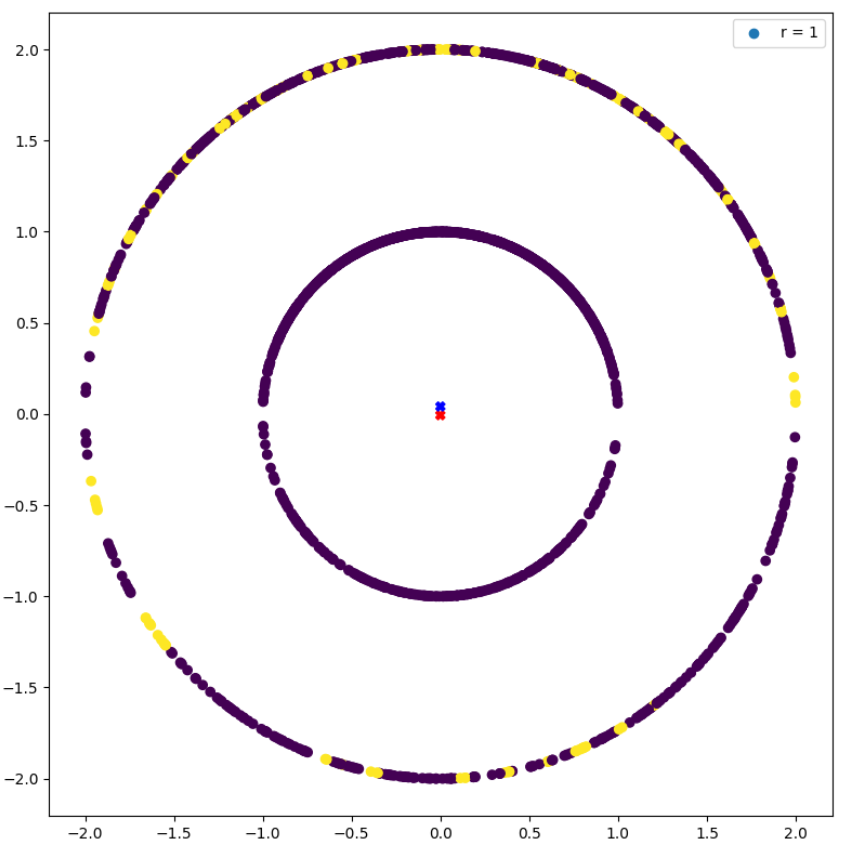
\includegraphics[width=1.9in]{figs/concentricr1.png}}%
\label{figure3a}
\hfil
\subfloat[r=2, rank=1717]{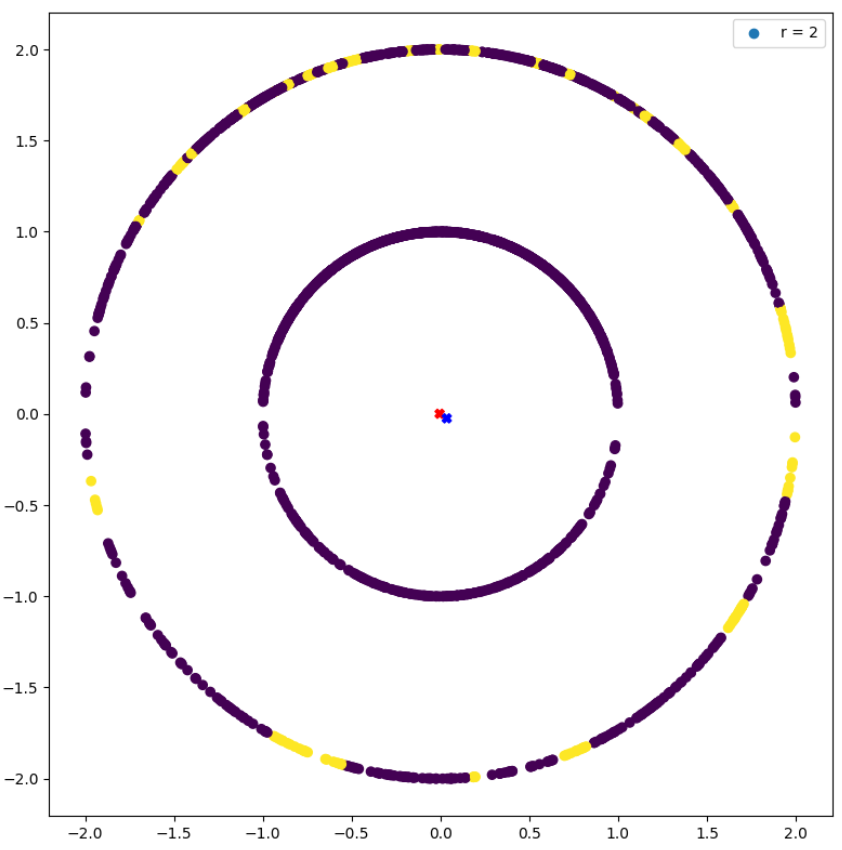
\includegraphics[width=1.9in]{figs/concentricr2.png}}%
\label{figure3a}
\hfil
\subfloat[r=3, rank=1891]{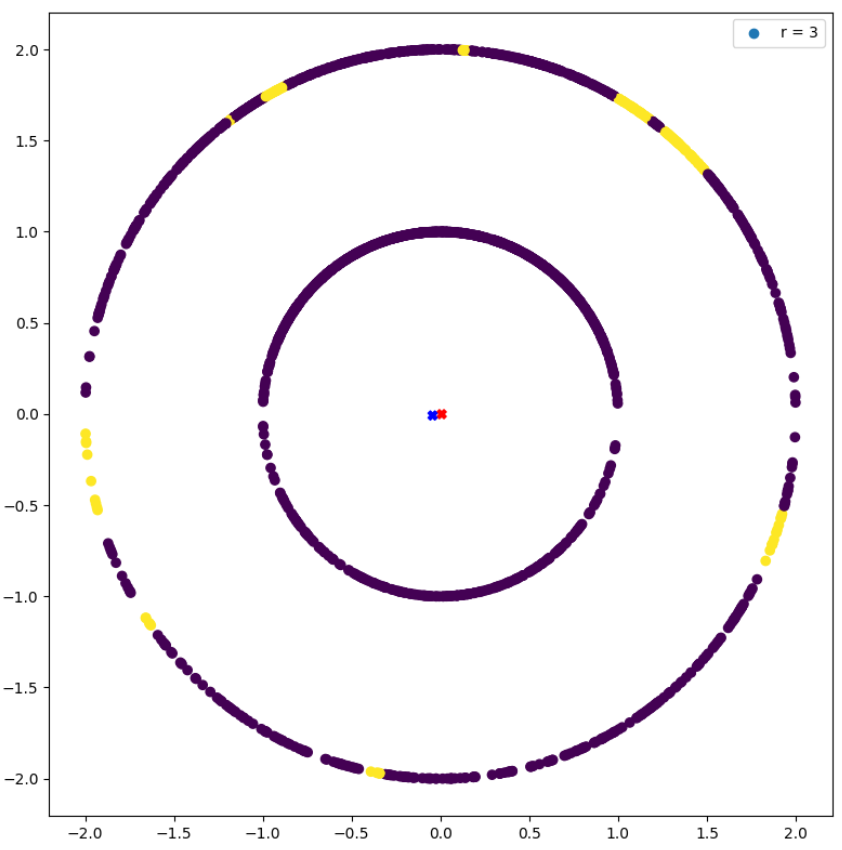
\includegraphics[width=1.9in]{figs/concentricr3.png}}%
\label{figure3a}
\hfil
\subfloat[r=4, rank=1952]{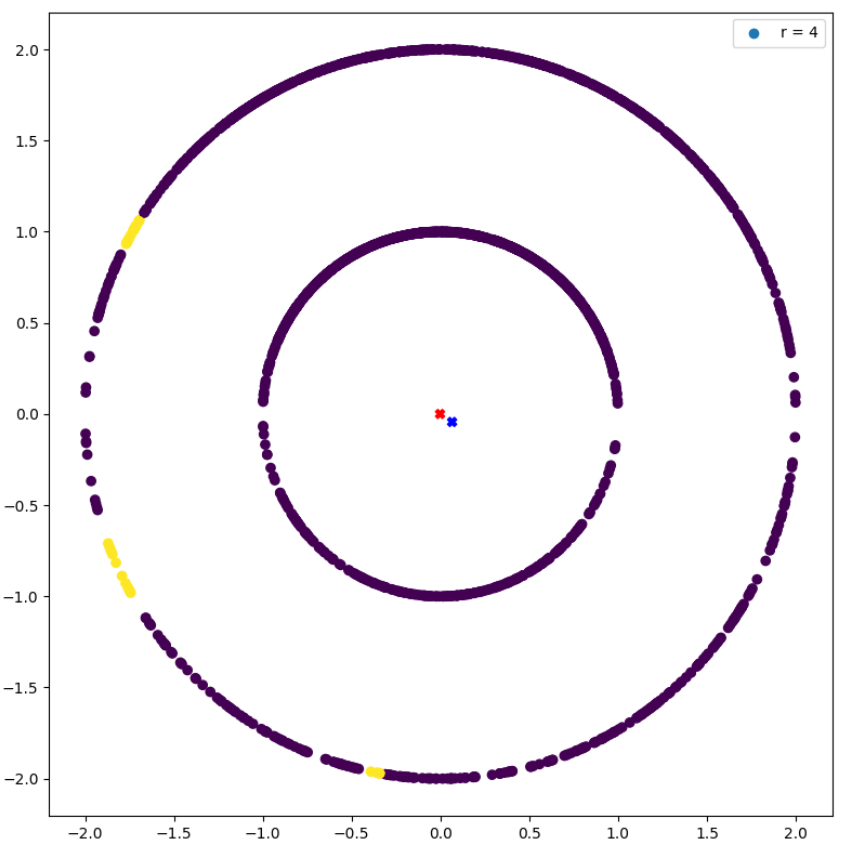
\includegraphics[width=1.9in]{figs/concentricr4.png}}%
\label{figure3a}
\hfil
\subfloat[r=5, rank=1983]{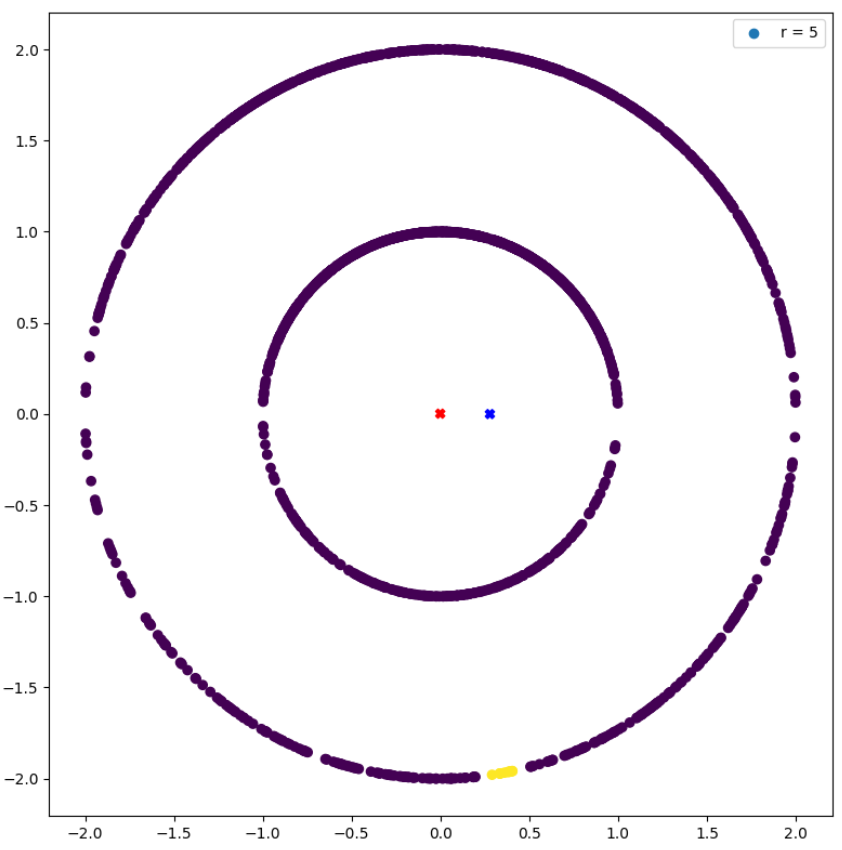
\includegraphics[width=1.9in]{figs/concentricr5.png}}%
\label{figure3b}
\hfil
\subfloat[r=6, rank=1996]{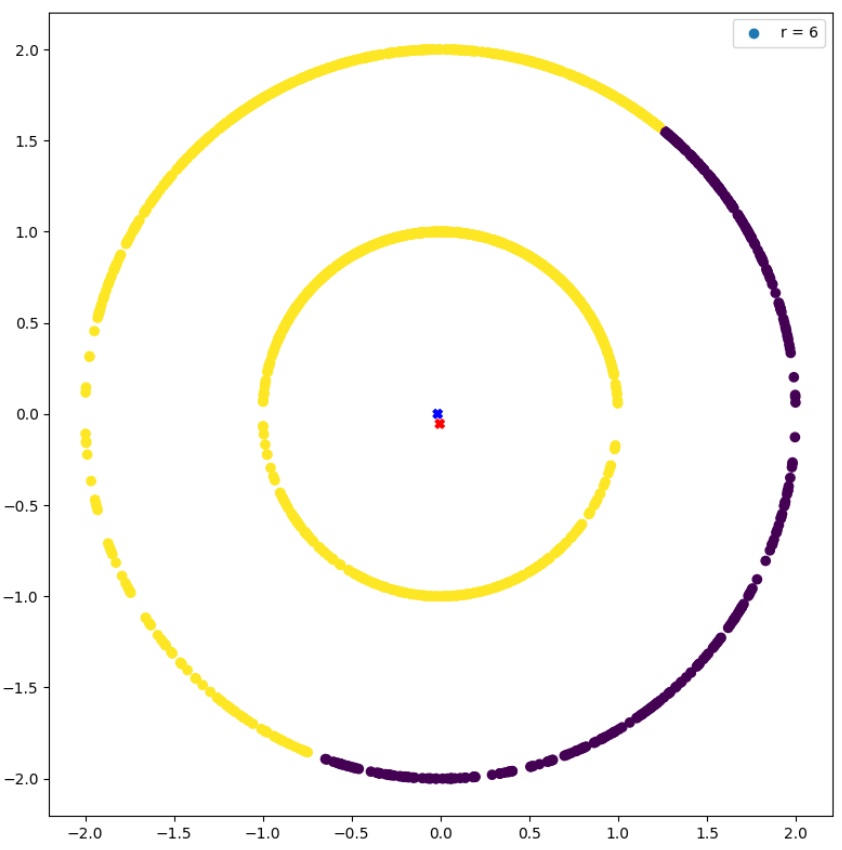
\includegraphics[width=1.9in]{figs/concentricr6.png}}%
\label{figure3a}
\hfil
\subfloat[r=7, rank=1997]{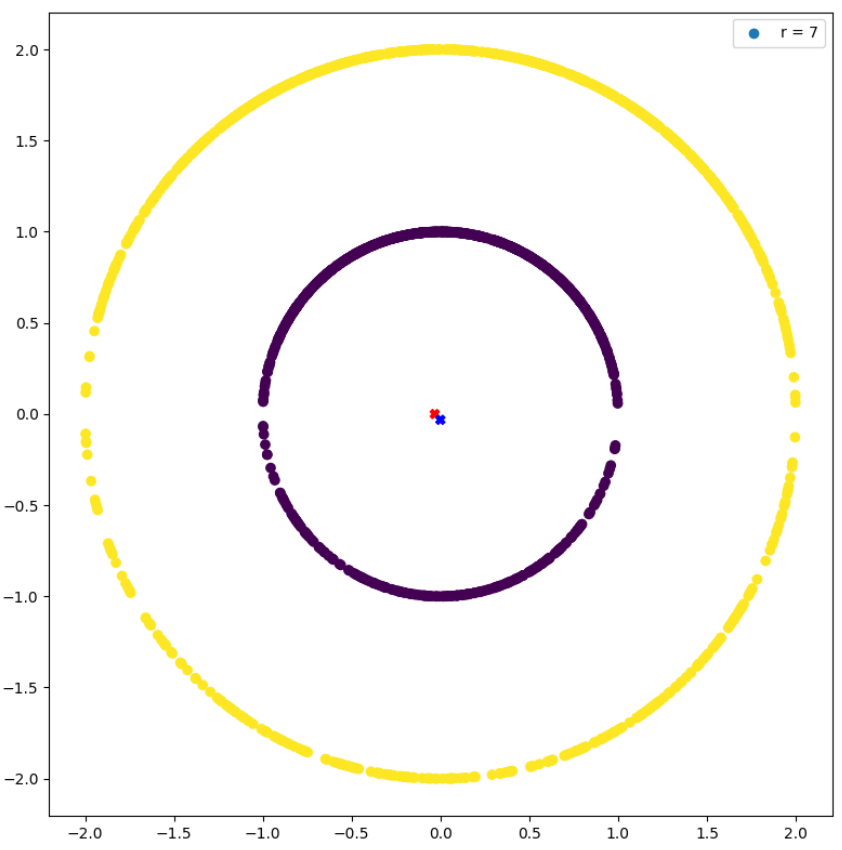
\includegraphics[width=1.9in]{figs/concentricr7.png}}%
\label{figure3c}
\hfil
\subfloat[r=8, rank=1997]{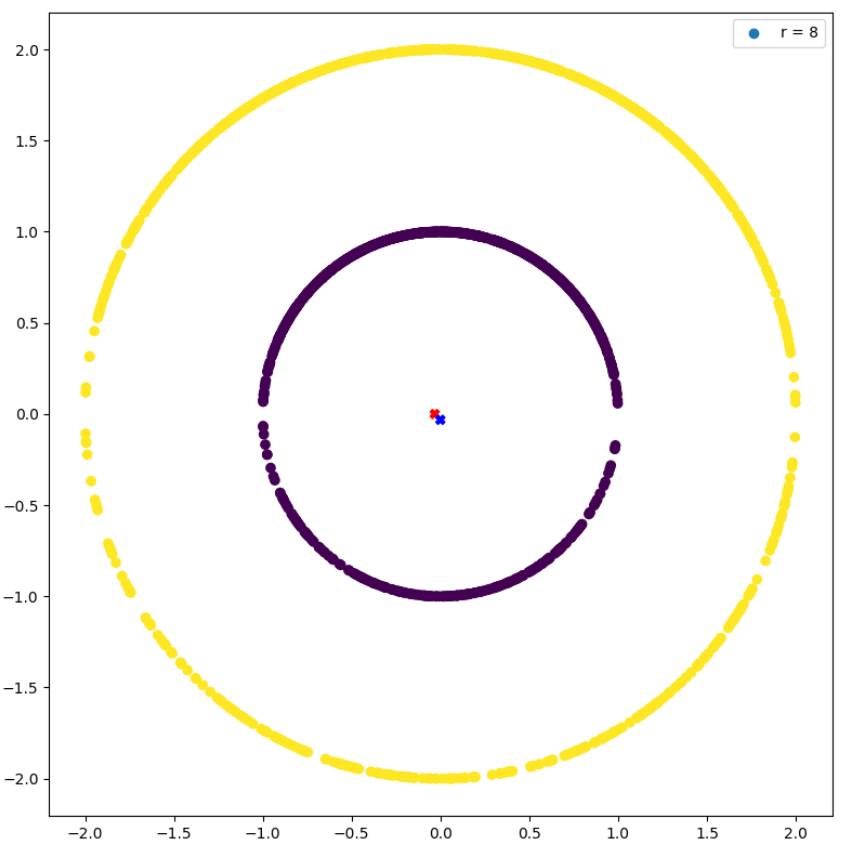
\includegraphics[width=1.9in]{figs/concentricr8.png}}%
\label{figure3a}
\hfil
\subfloat[r=9, rank=1997]{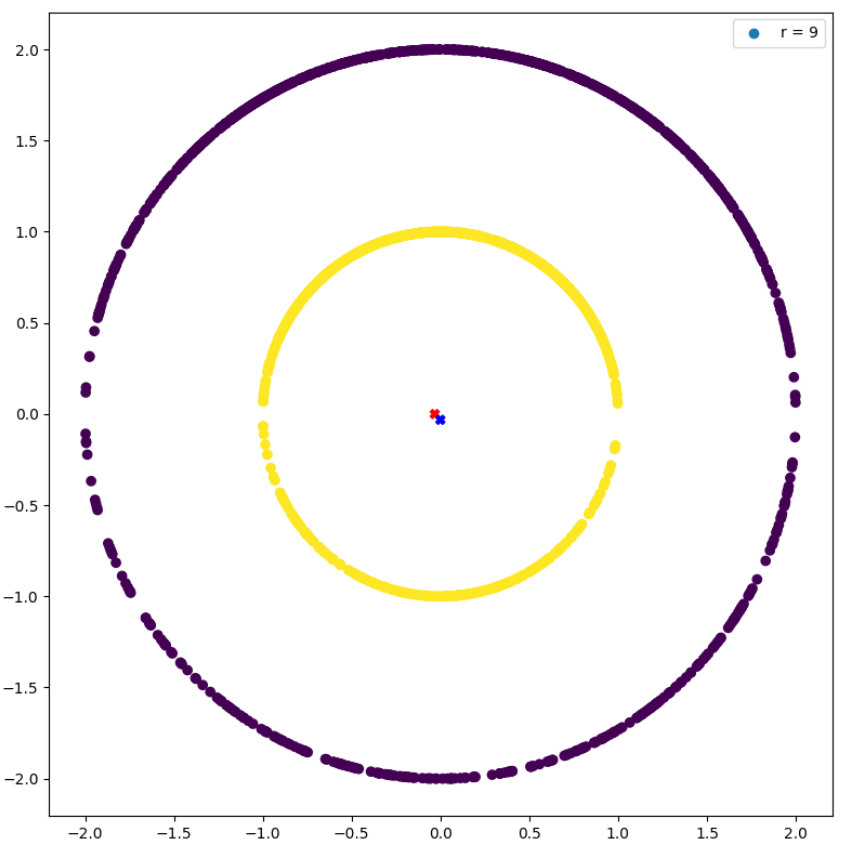
\includegraphics[width=1.9in]{figs/concentricr9.png}}%
\label{figure3d}
\hfil
\caption{Concentric datasets after flexible k-means (for r = 1 $\sim$ 9, data size=1999)}
\end{figure*}\newpage
\begin{figure*}[!h]
\centering
\subfloat[r=100, rank=1998]{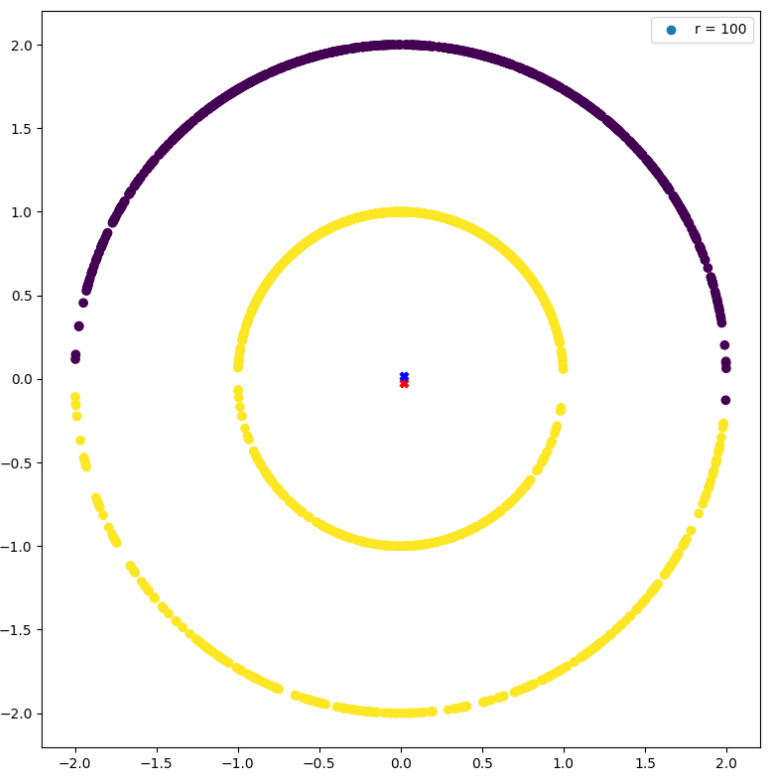
\includegraphics[width=1.9in]{figs/concentric100.png}}%
\label{figure3c}
\hfil
\subfloat[r=200, rank=1998]{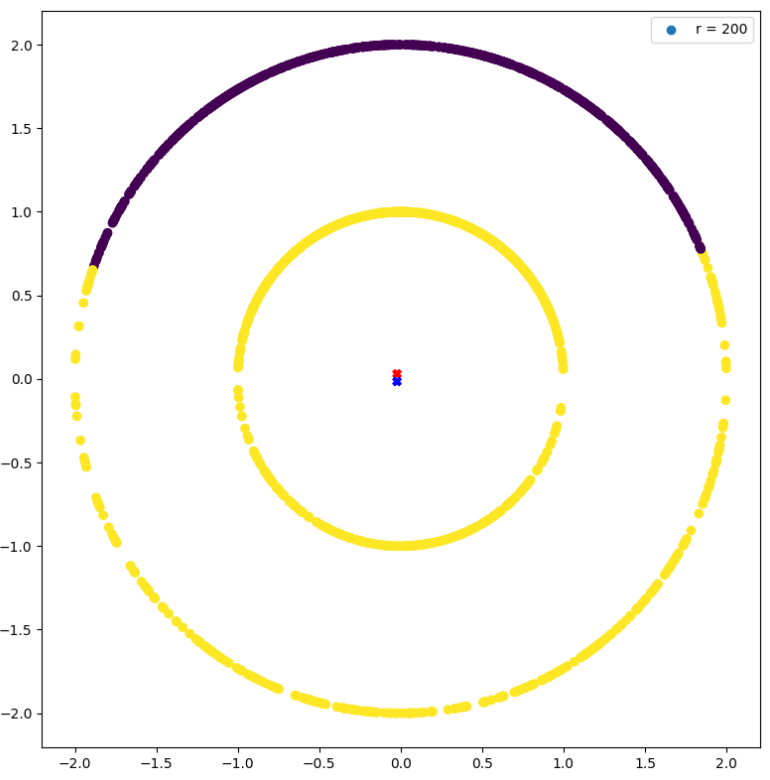
\includegraphics[width=1.9in]{figs/concentric200.png}}%
\label{figure3a}
\hfil
\subfloat[r=300, rank=1998]{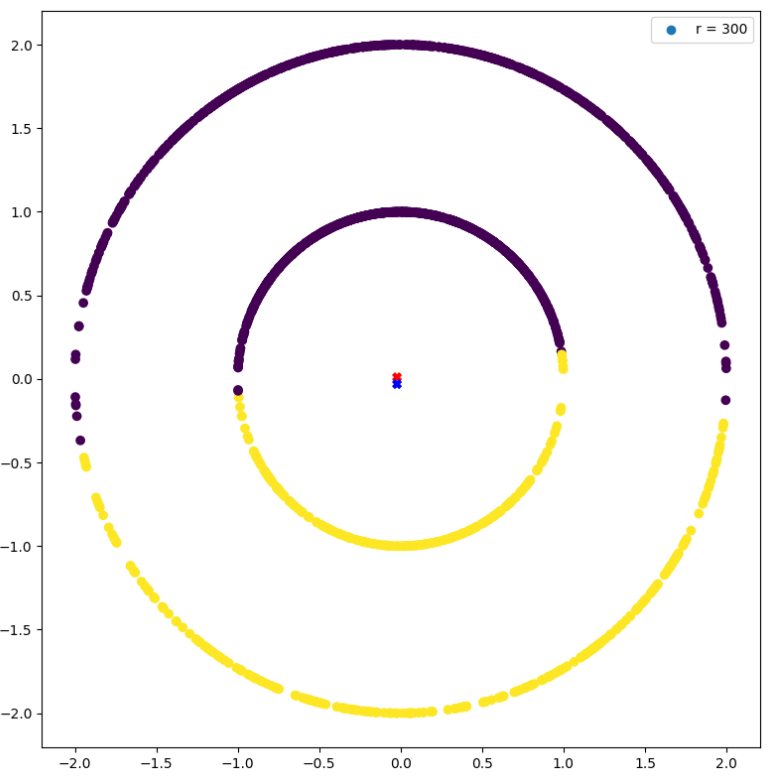
\includegraphics[width=1.9in]{figs/concentric300.png}}%
\caption{Concentric datasets after flexible k-means (for r = 100, 200, 300, data size=1999)}
\end{figure*}
\begin{figure*}[!htbp]
\centering
\subfloat[r=1, rank=279]{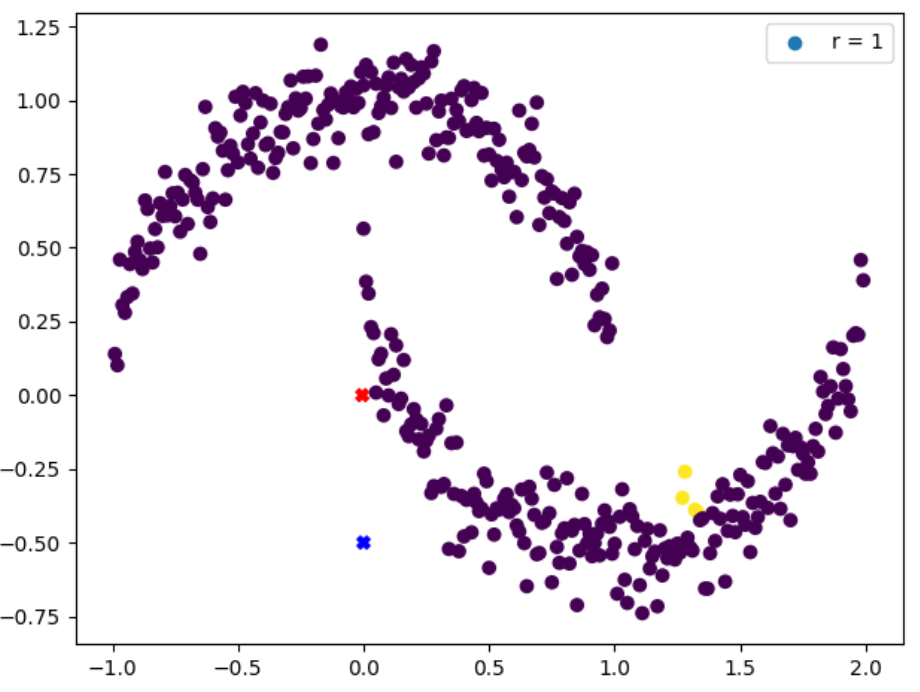
\includegraphics[width=2in]{figs/nonsphericalr1.png}}%
\label{figure3a}
\hfil
\subfloat[r=2, rank=376]{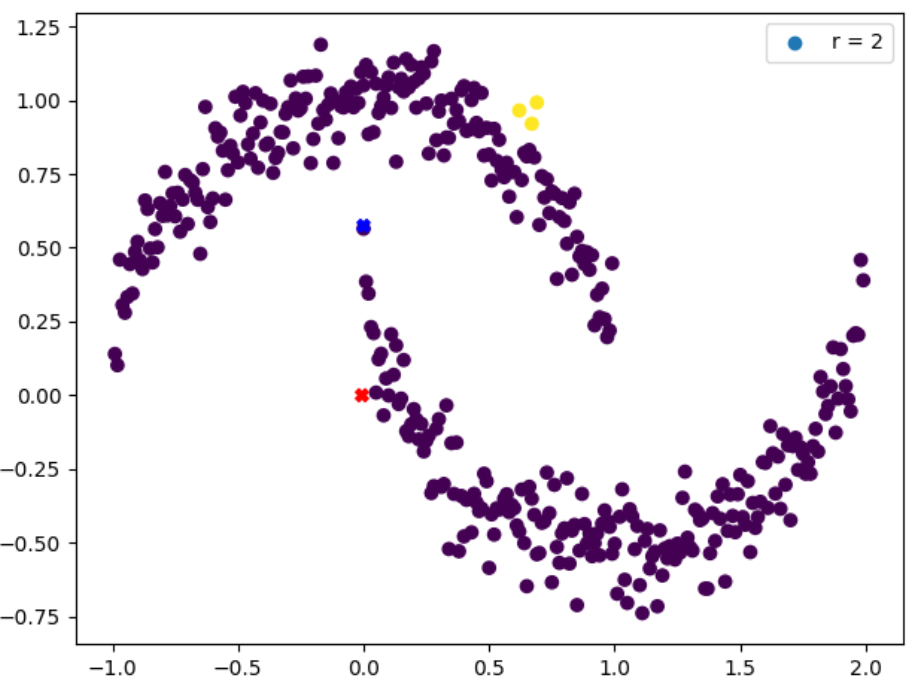
\includegraphics[width=2in]{figs/nonsphericalr2.png}}%
\label{figure3b}
\hfil
\subfloat[r=3, rank=393]{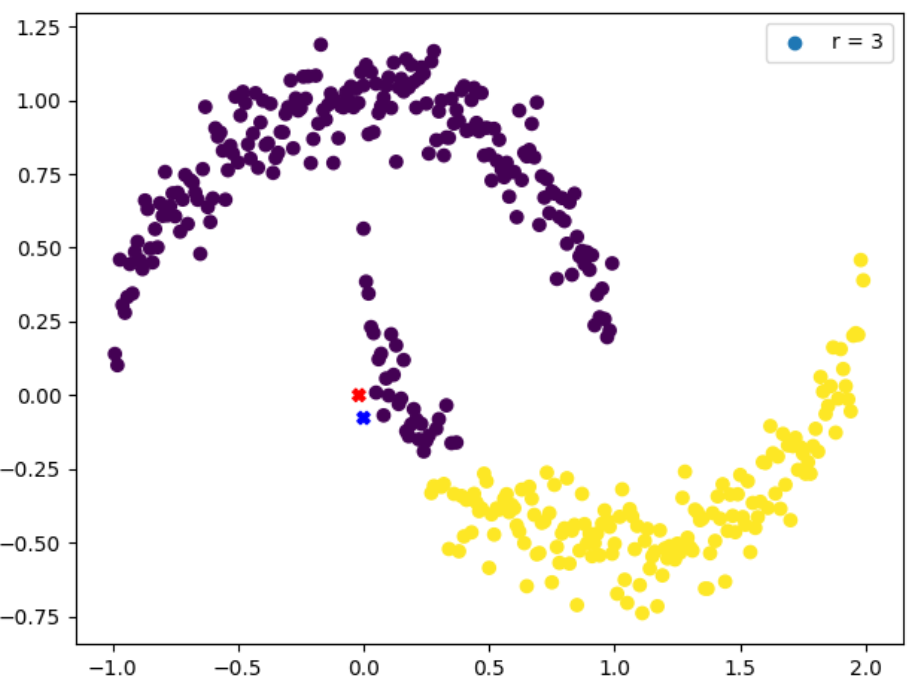
\includegraphics[width=2in]{figs/nonsphericalr3.png}}%
\label{figure3c}
\hfil
\subfloat[r=4, rank=397]{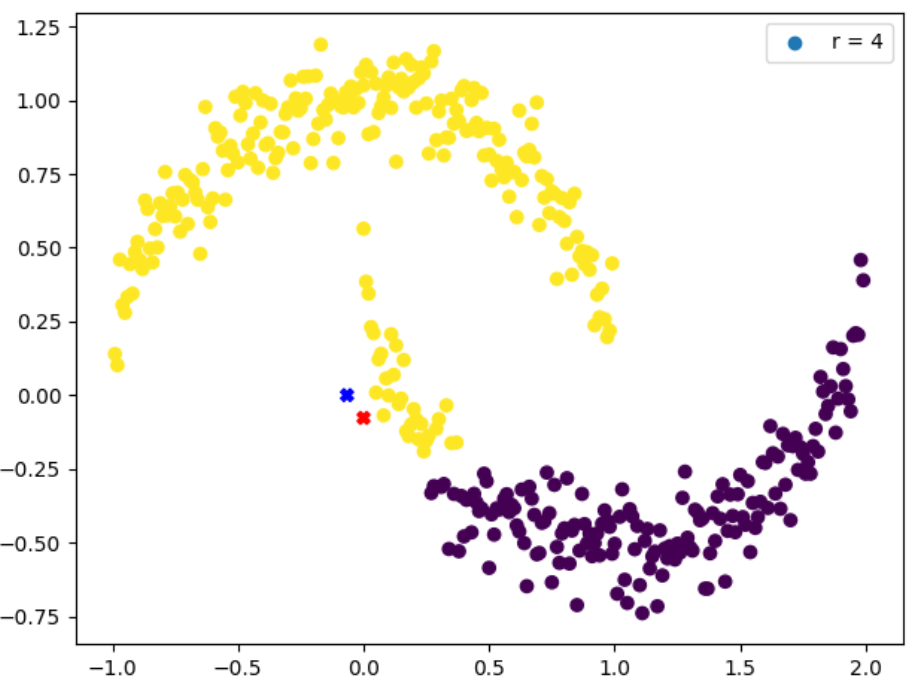
\includegraphics[width=2in]{figs/nonsphericalr4.png}}%
\label{figure3d}
\hfil
\subfloat[r=5, rank=398]{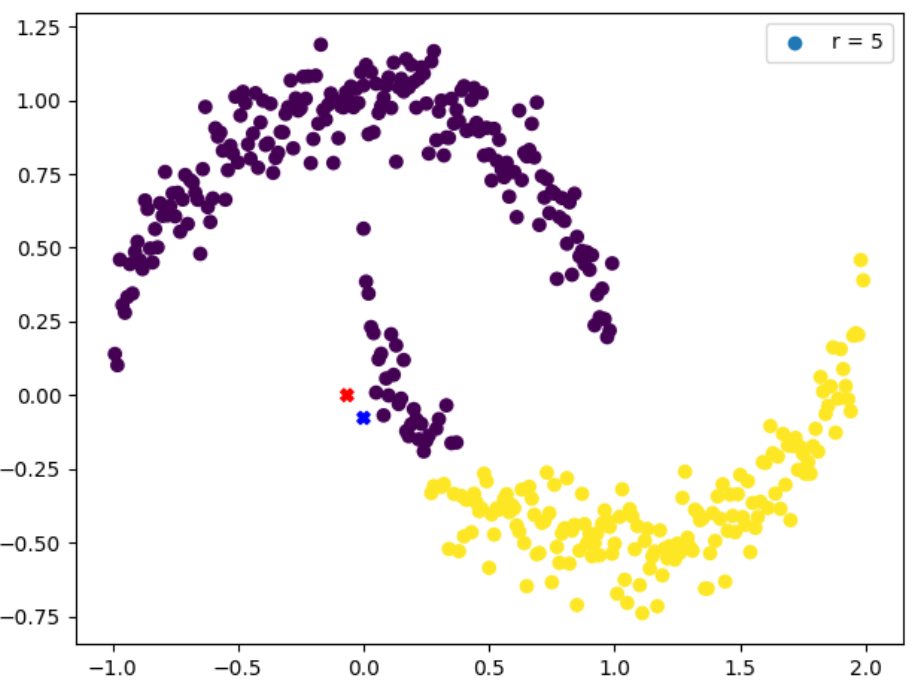
\includegraphics[width=2in]{figs/nonsphericalr5.png}}%
\label{figure3e}
\hfil
\subfloat[r=6, rank=398]{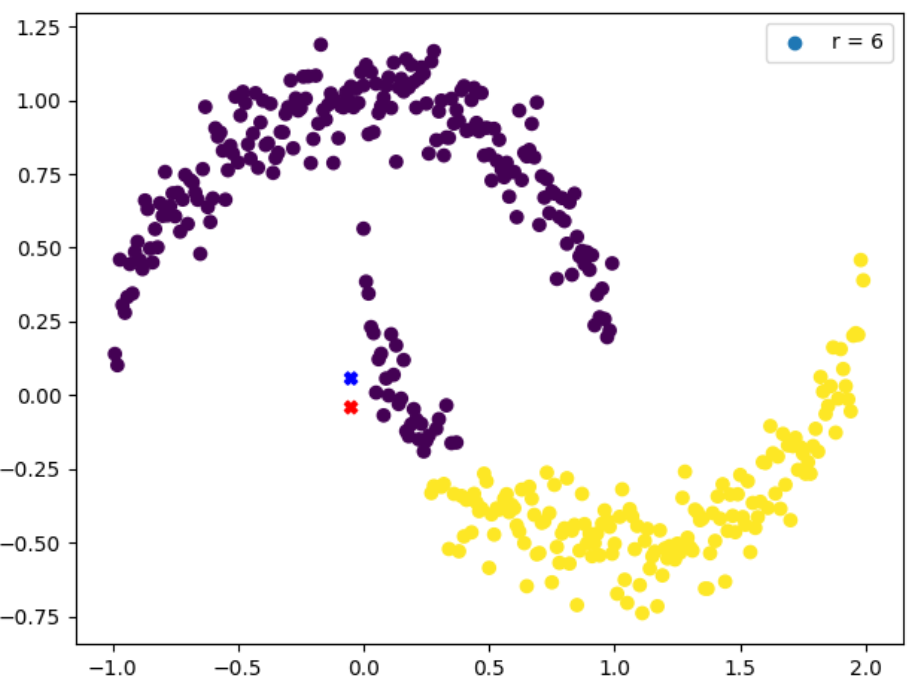
\includegraphics[width=2in]{figs/nonsphericalr6.png}}%
\label{figure3g}
\hfil
\subfloat[r=7, rank=398]{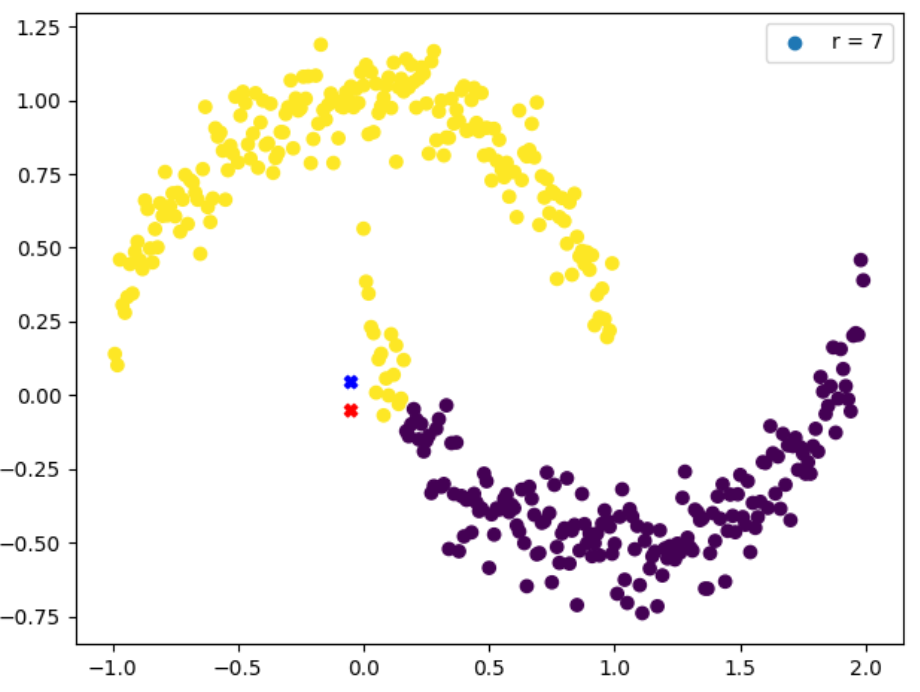
\includegraphics[width=2in]{figs/nonsphericalr7.png}}%
\label{figure3h}
\hfil
\subfloat[r=8, rank=398]{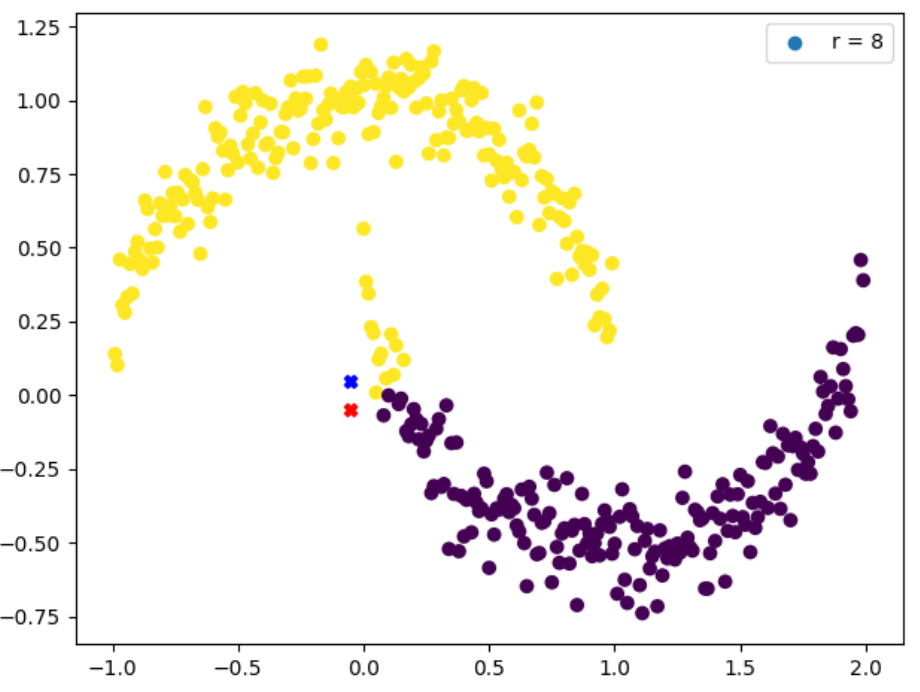
\includegraphics[width=2in]{figs/nonsphericalr8.png}}%
\label{figure3k}
\hfil
\subfloat[r=9, rank=398]{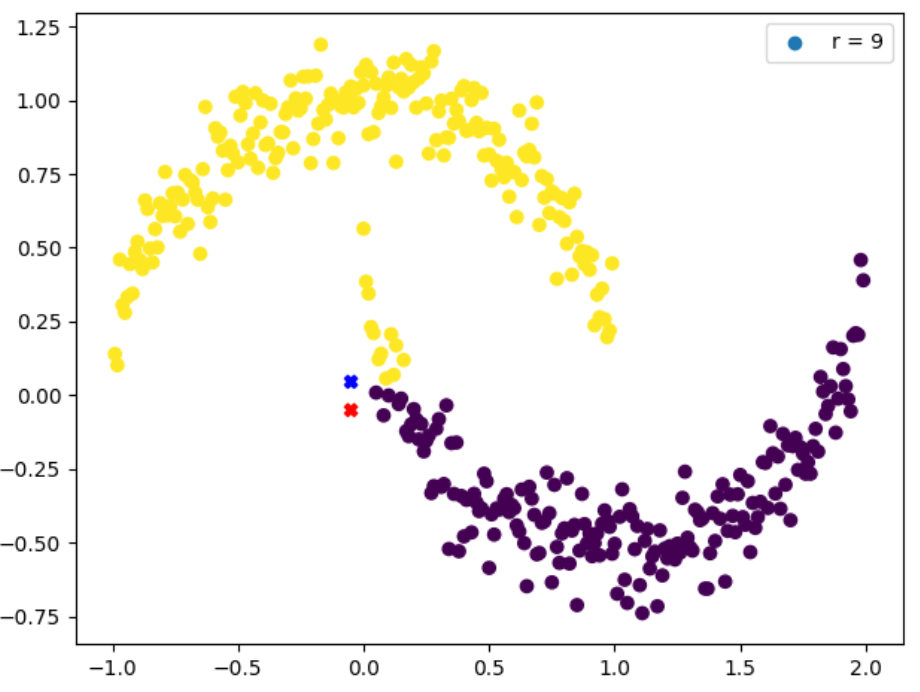
\includegraphics[width=2in]{figs/nonsphericalr9.png}}%
\label{figure3k}
\caption{Non-spherical datasets after flexible k-means (for r = 1 $\sim$ 9, data size=399)}
\end{figure*}

\begin{figure*}[!htbp]
\centering
\subfloat[r=9, rank=398]{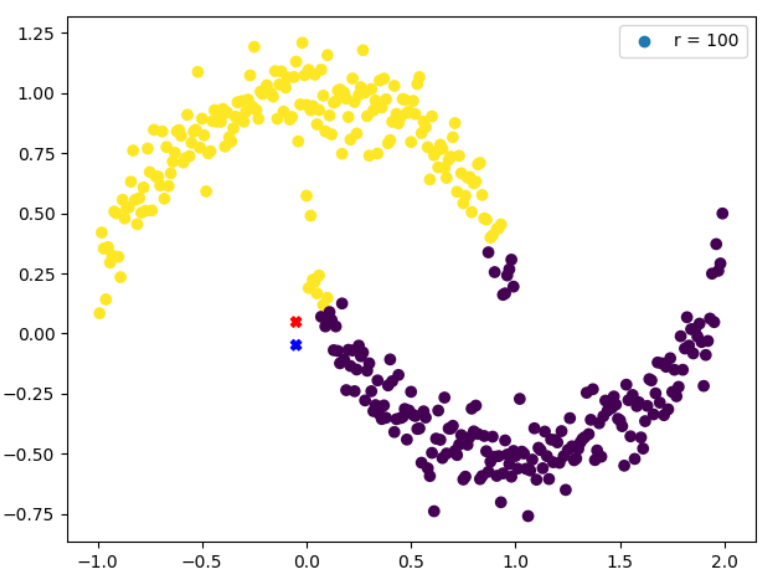
\includegraphics[width=2in]{figs/nonsphericalr100.png}}%
\label{figure3k}
\subfloat[r=9, rank=398]{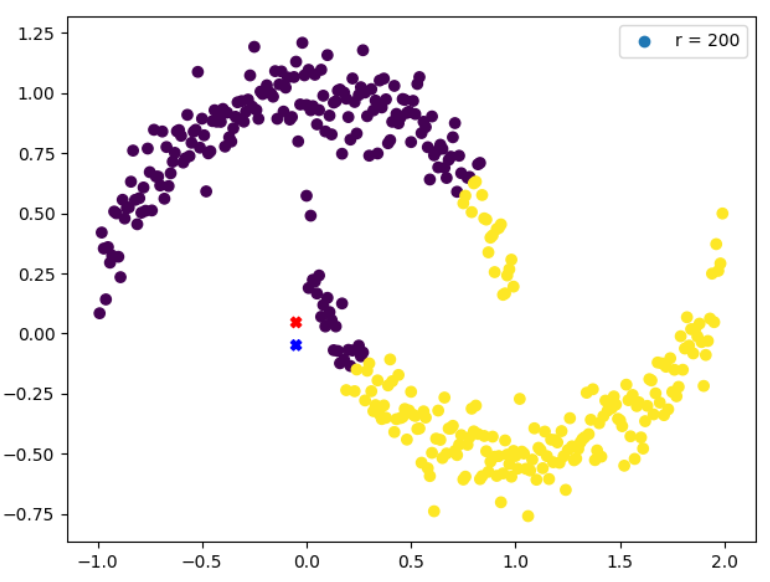
\includegraphics[width=2in]{figs/nonsphericalr200.png}}%
\label{figure3k}
\subfloat[r=9, rank=398]{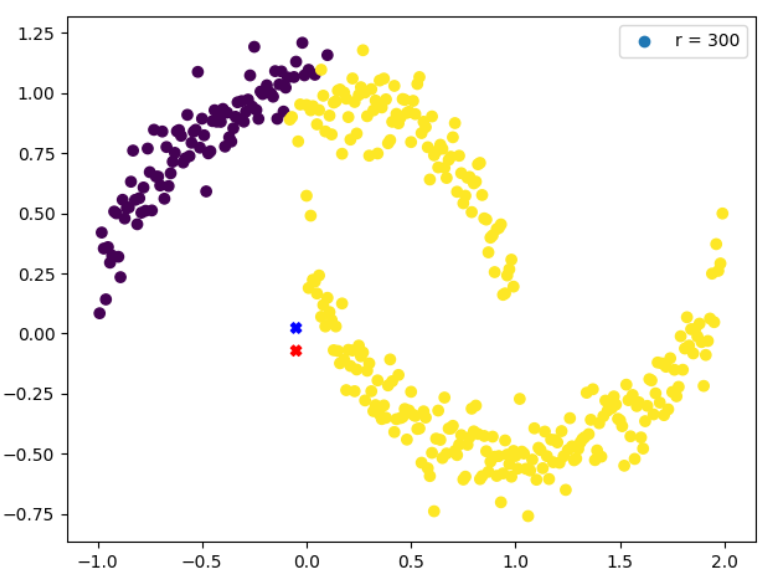
\includegraphics[width=2in]{figs/nonsphericalr300.png}}%
\label{figure3k}
\caption{Non-spherical datasets after flexible k-means (for r = 100, 200, 300, data size=399)}
\end{figure*}

\begin{figure*}[!htbp]
\centering
\subfloat[r=1, rank=361]{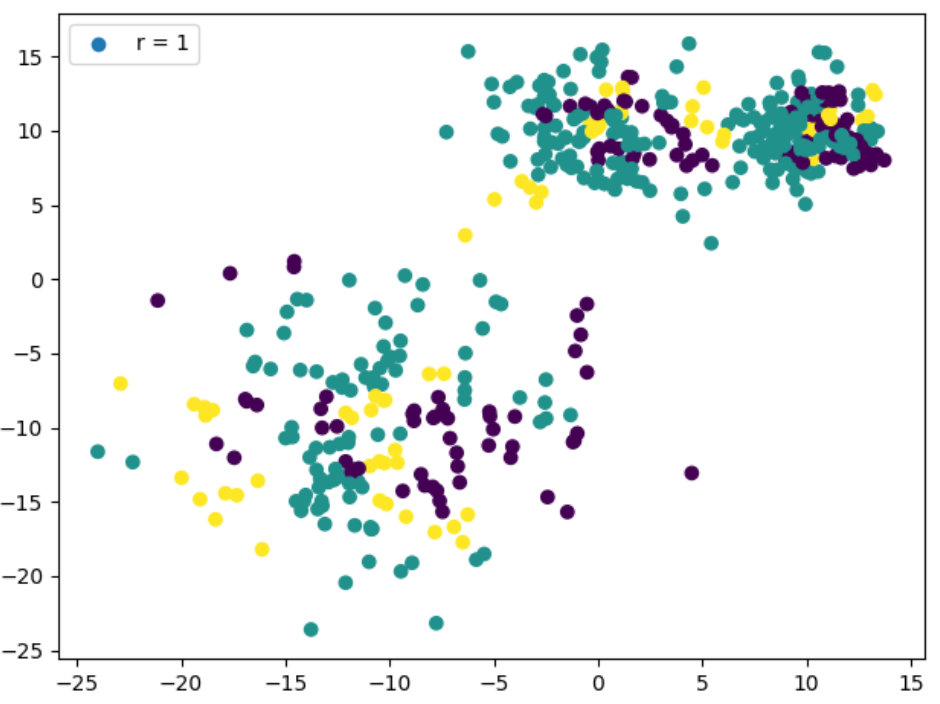
\includegraphics[width=2in]{figs/gmmr1.png}}%
\label{figure3a}
\hfil
\subfloat[r=2, rank=478]{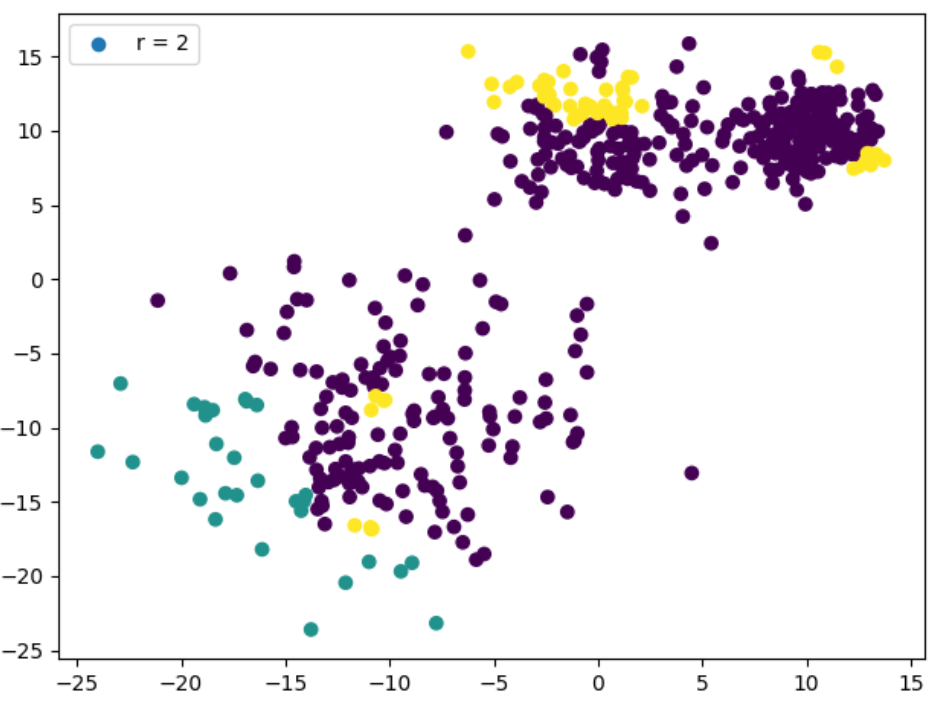
\includegraphics[width=2in]{figs/gmmr2.png}}%
\label{figure3b}
\hfil
\subfloat[r=3, rank=497]{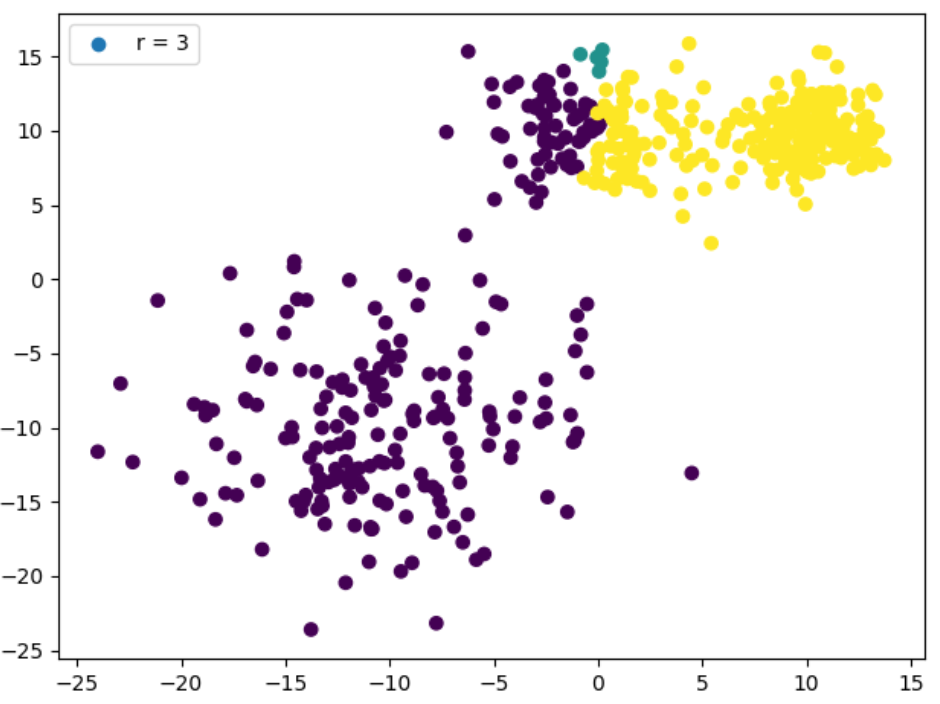
\includegraphics[width=2in]{figs/gmmr3.png}}%
\label{figure3c}
\hfil
\subfloat[r=4, rank=498]{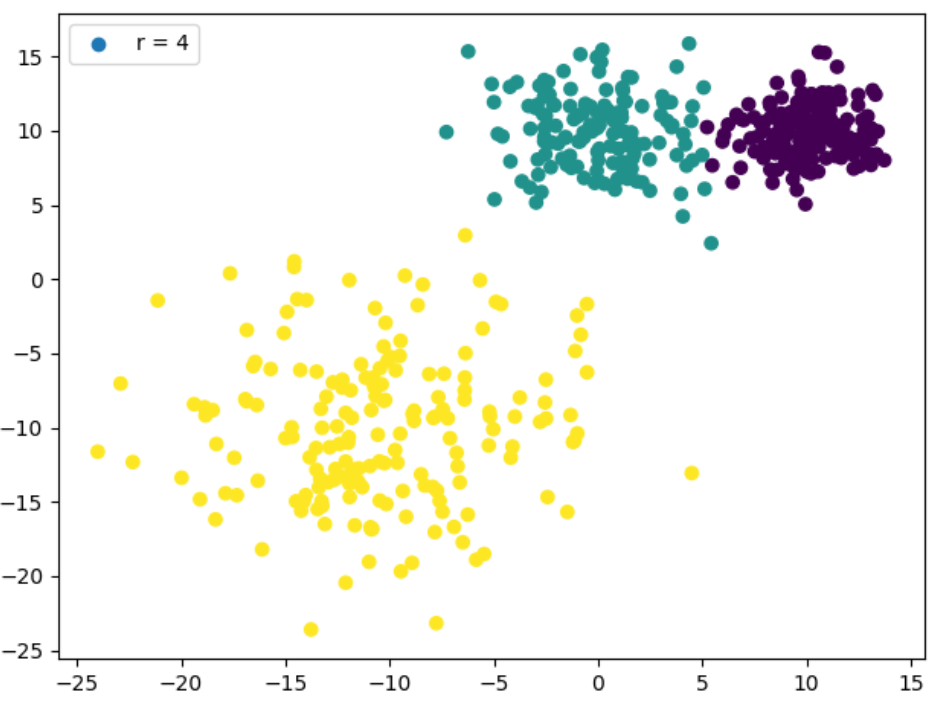
\includegraphics[width=2in]{figs/gmmr4.png}}%
\label{figure3d}
\hfil
\subfloat[r=5, rank=498]{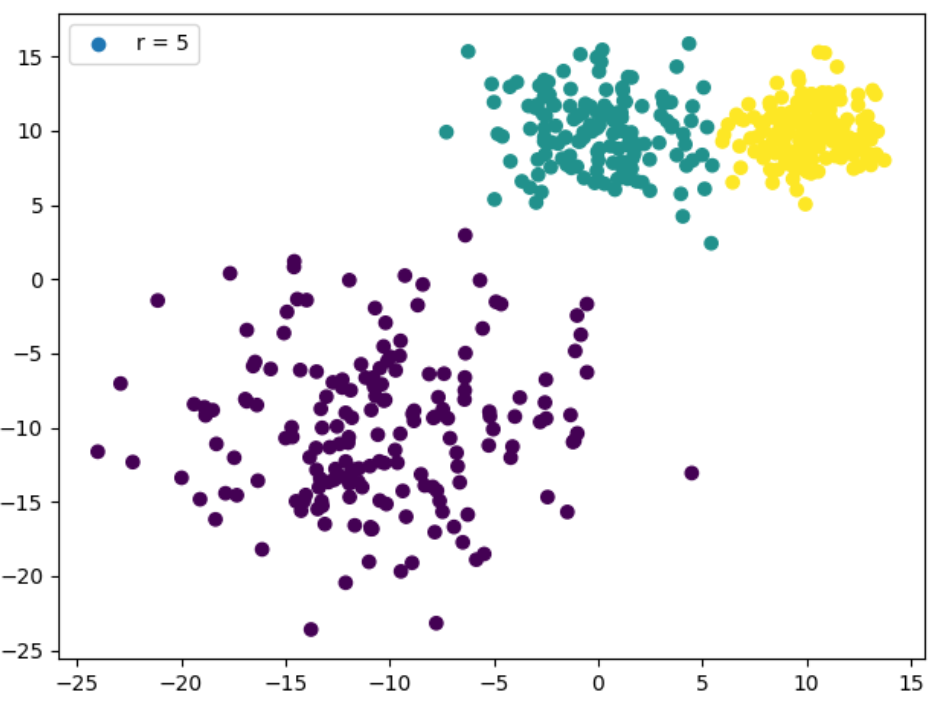
\includegraphics[width=2in]{figs/gmmr5.png}}%
\label{figure3e}
\hfil
\subfloat[r=6, rank=498]{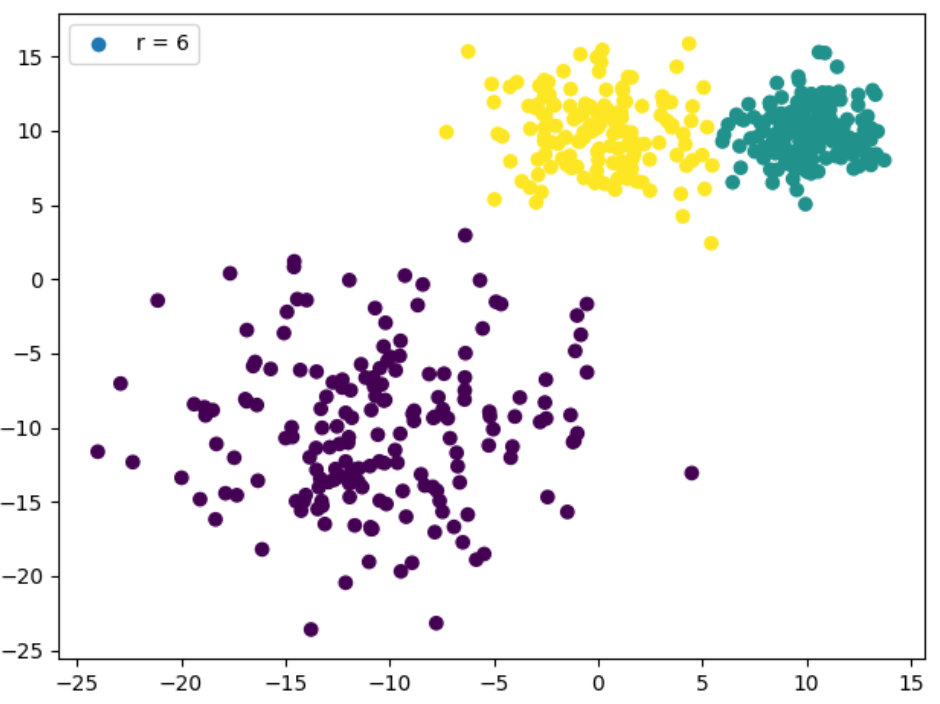
\includegraphics[width=2in]{figs/gmmr6.png}}%
\label{figure3f}
\hfil
\subfloat[r=7, rank=498]{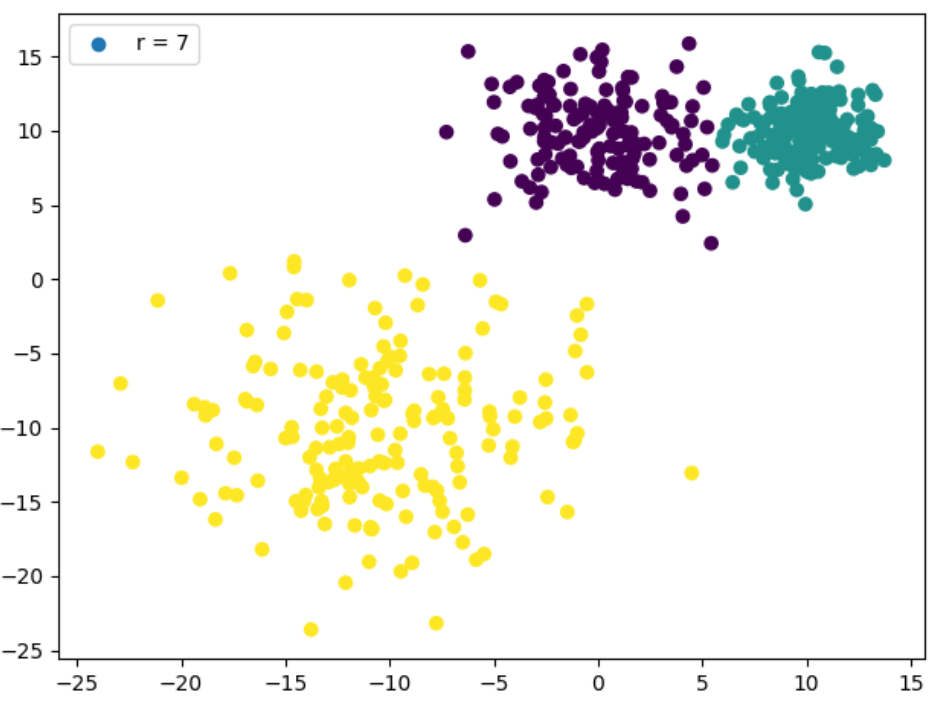
\includegraphics[width=2in]{figs/gmmr7.png}}%
\label{figure3g}
\hfil
\subfloat[r=8, rank=498]{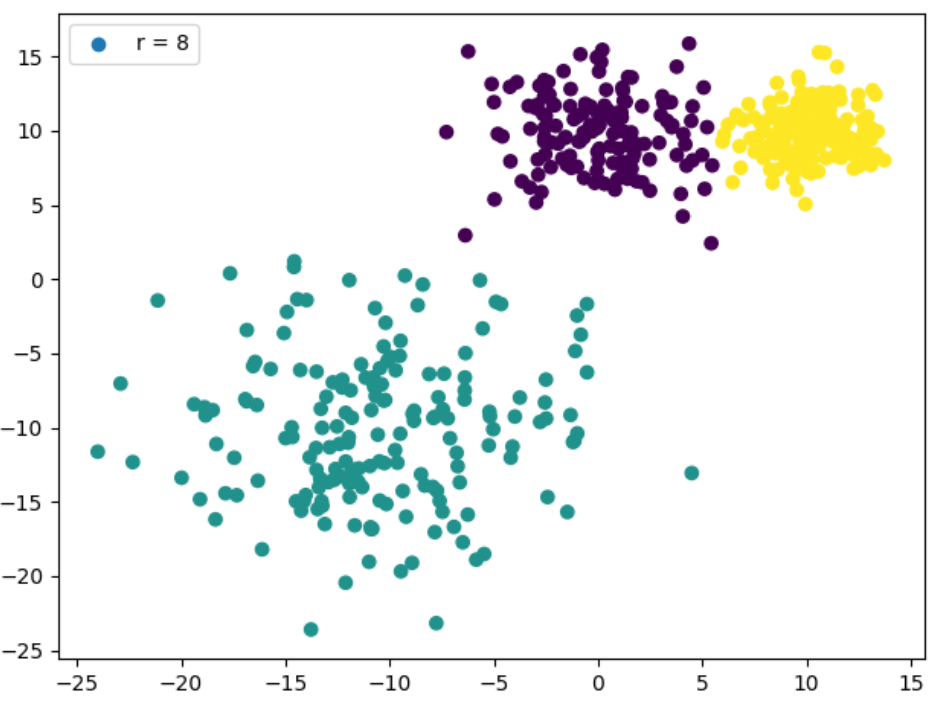
\includegraphics[width=2in]{figs/gmmr8.png}}%
\label{figure3h}
\hfil
\subfloat[r=9, rank=498]{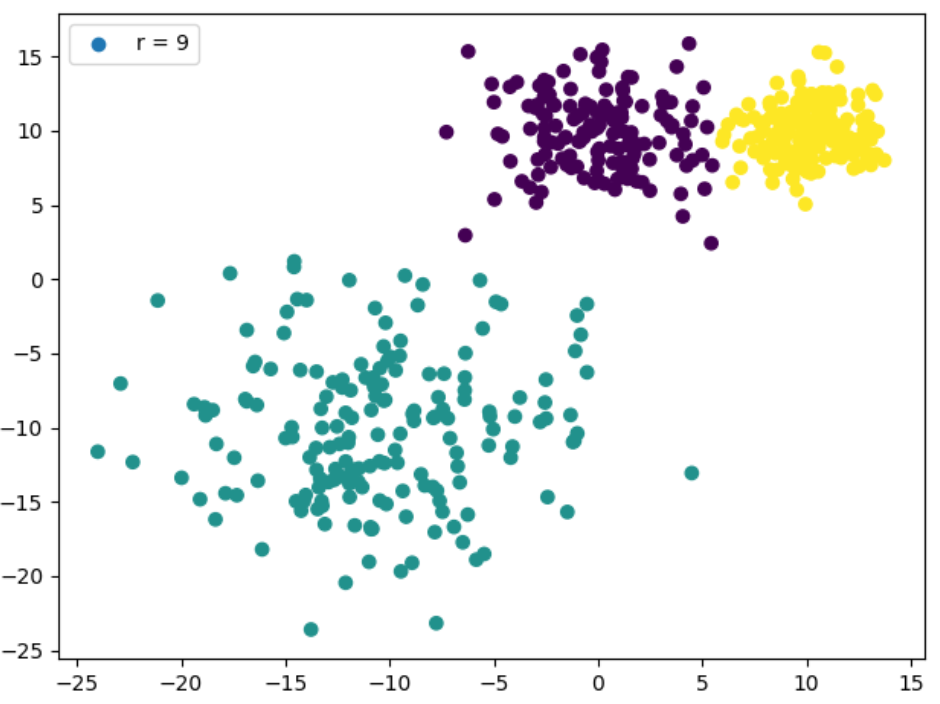
\includegraphics[width=2in]{figs/gmmr9.png}}%
\label{figure3k}
\caption{GMM datasets after flexible k-means (for r = 1 $\sim$ 9, data size=499)}
\end{figure*}
\begin{figure*}[ht]
\centering
\subfloat[r=100, rank=498]{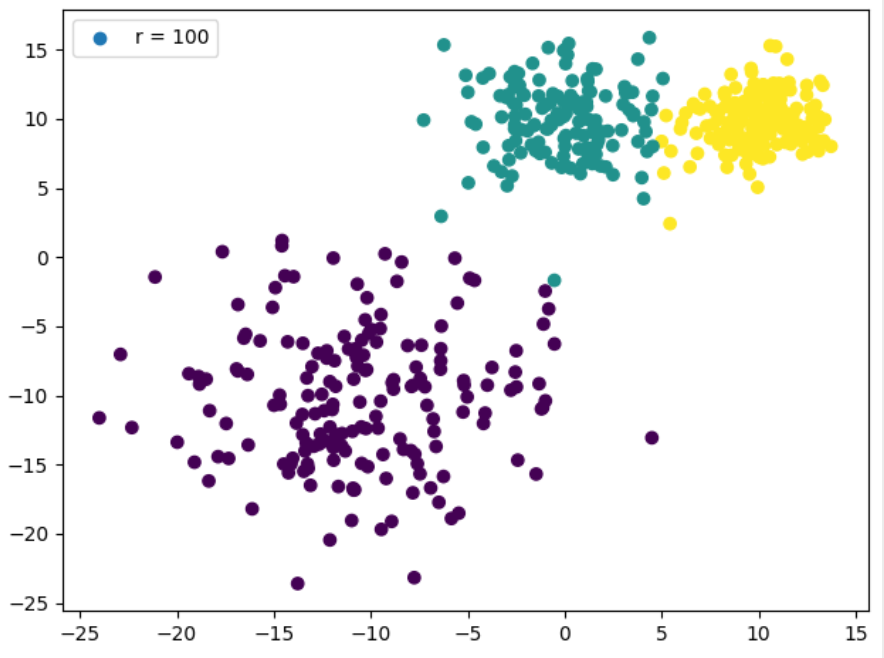
\includegraphics[width=2.5in]{figs/gmmr100.png}}%
\label{figure3a}
\hfil
\subfloat[r=200, rank=498]{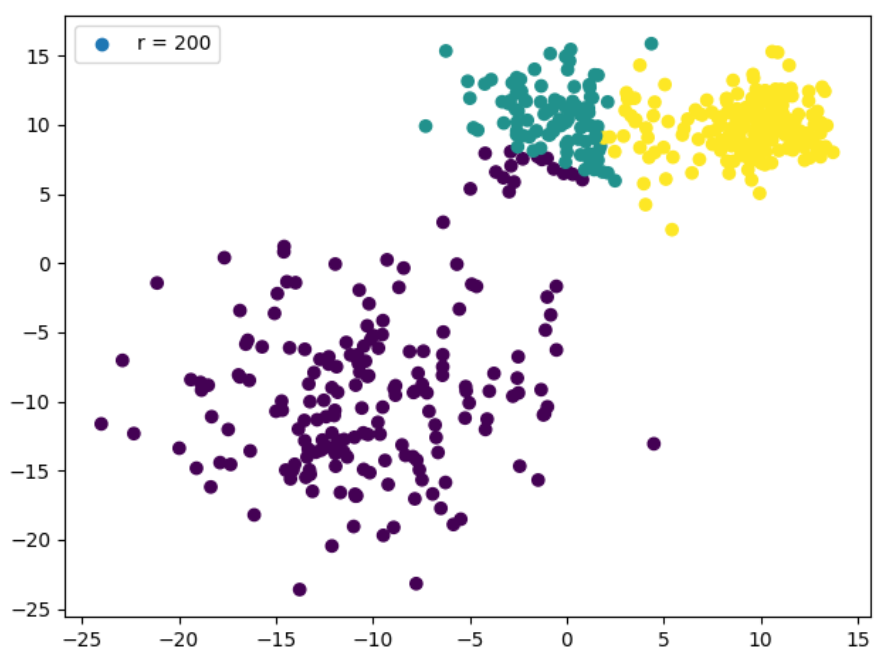
\includegraphics[width=2.5in]{figs/gmmr200.png}}%
\label{figure3b}
\hfil
\subfloat[r=300, rank=498]{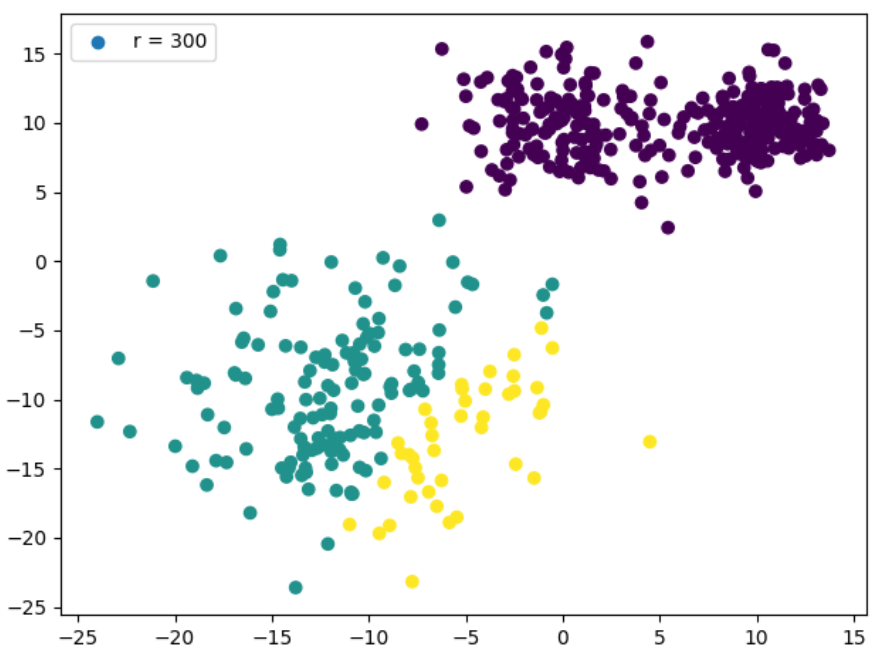
\includegraphics[width=2.5in]{figs/gmmr300.png}}%
\label{figure3c}
\hfil
\subfloat[r=400, rank=498]{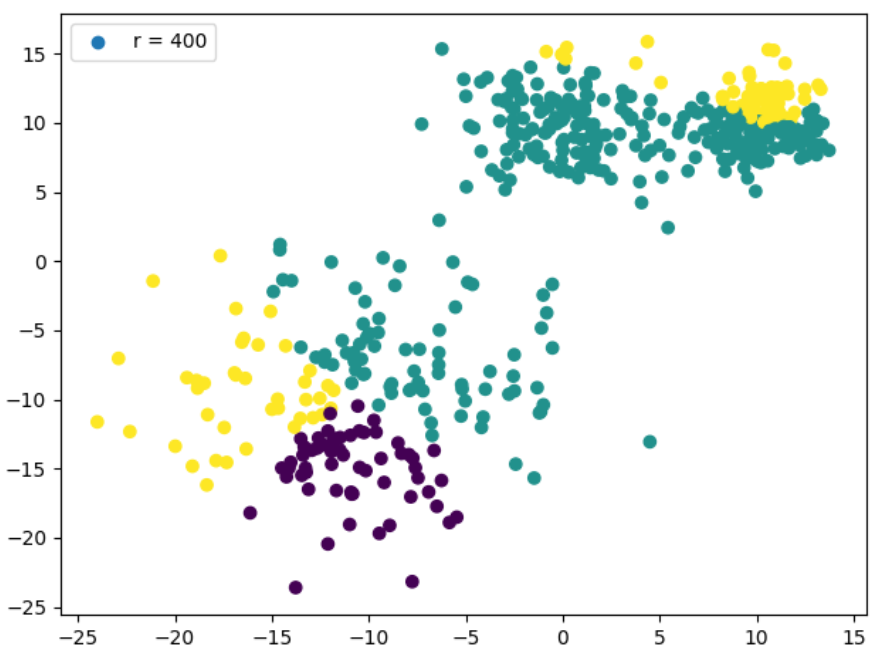
\includegraphics[width=2.5in]{figs/gmmr400.png}}%
\label{figure3d}
\caption{GMM datasets after flexible k-means (for r = 100 $\sim$ 900, data size=499)}
\end{figure*}

\begin{figure*}[!htbp]
\centering
\subfloat[r=1, rank=794]{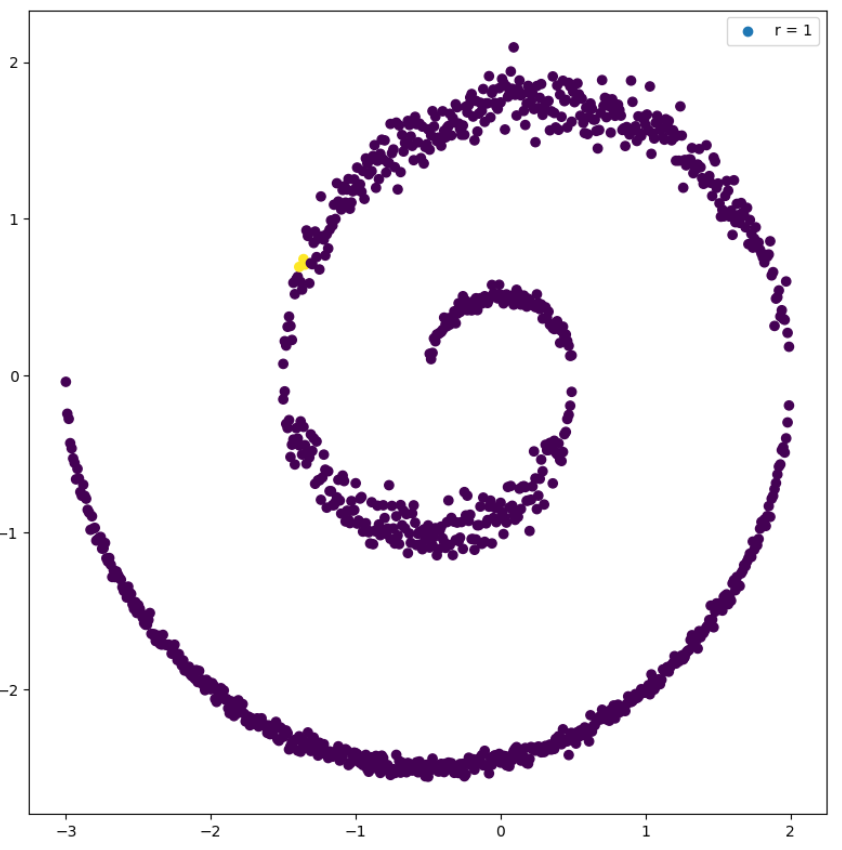
\includegraphics[width=2in]{figs/spiralr1.png}}%
\label{figure3a}
\hfil
\subfloat[r=2, rank=1074]{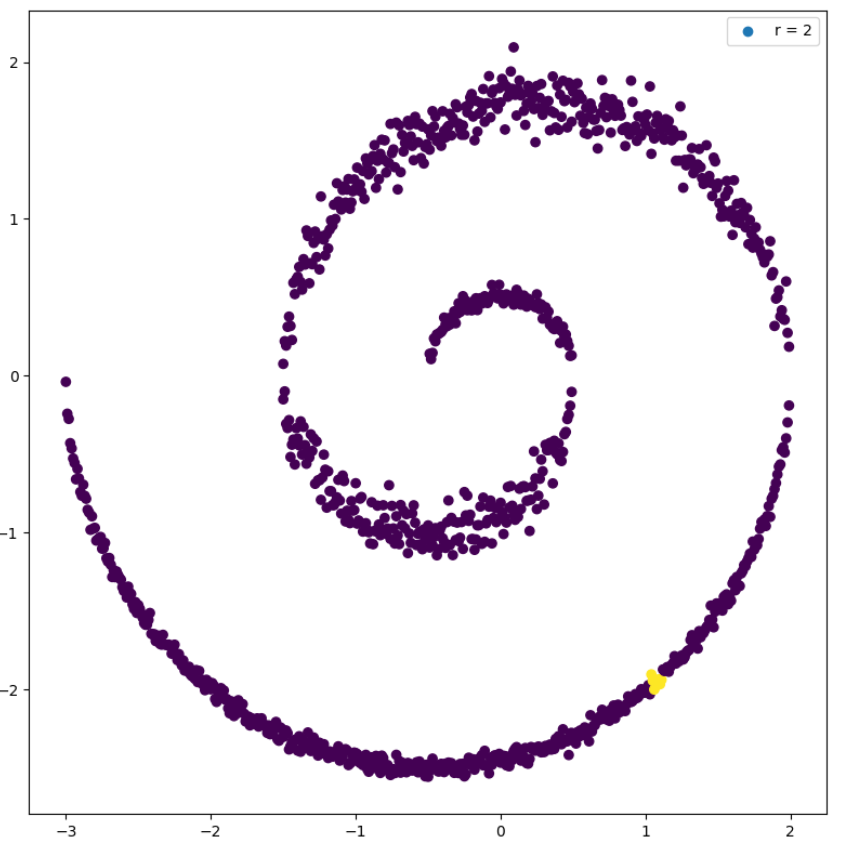
\includegraphics[width=2in]{figs/spiralr2.png}}%
\label{figure3a}
\hfil
\subfloat[r=3, rank=1134]{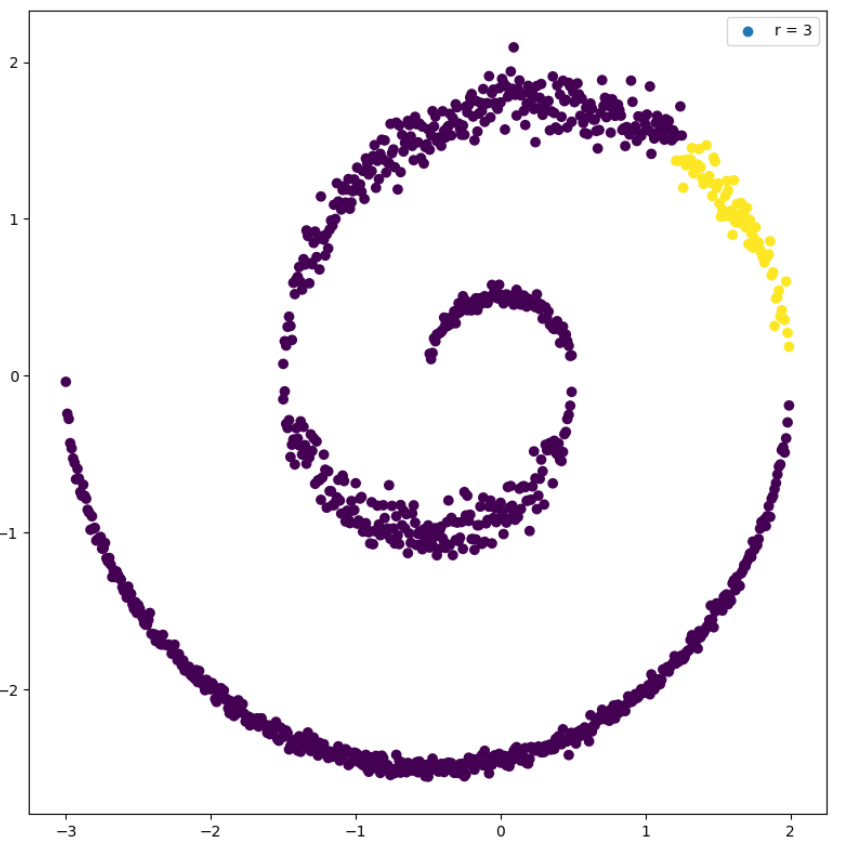
\includegraphics[width=2in]{figs/spiralr3.png}}%
\label{figure3b}
\hfil
\subfloat[r=4, rank=1142]{\includegraphics[width=2in]{figs/spiralr4.png}}%
\label{figure3c}
\hfil
\subfloat[r=5, rank=1146]{\includegraphics[width=2in]{figs/spiralr5.png}}%
\label{figure3d}
\hfil
\subfloat[r=6, rank=1148]{\includegraphics[width=2in]{figs/spiralr6.png}}%
\label{figure3e}
\hfil
\subfloat[r=7, rank=1148]{\includegraphics[width=2in]{figs/spiralr7.png}}%
\label{figure3g}
\hfil
\subfloat[r=8, rank=1148]{\includegraphics[width=2in]{figs/spiralr8.png}}%
\label{figure3h}
\hfil
\subfloat[r=9, rank=1148]{\includegraphics[width=2in]{figs/spiralr9.png}}%
\label{figure3k}
\caption{Spiral datasets after flexible k-means (for r = 1 $\sim$ 9)}
\end{figure*}

\begin{figure*}[!htbp]
\centering
\subfloat[r=100, rank=1148]{\includegraphics[width=2in]{figs/spiralr100.png}}%
\label{figure3k}
\subfloat[r=500, rank=1148]{\includegraphics[width=2in]{figs/spiralr500.png}}%
\label{figure3k}
\subfloat[r=1000, rank=1148]{\includegraphics[width=2in]{figs/spiralr1000.png}}%
\label{figure3k}
\caption{Spiral datasets after flexible k-means (for r = 100, 200, 300)}
\end{figure*}
\newpage 
%%%%%%%%%%%%%%%%%%%%%%%%%%%%%%%%%Problem 3%%%%%%%%%%%%%%%%%%%%%%%%%%%%%%%%%
\section*{Problem 3}
\subsection*{(i)}
The derivative of the discrepancy function $F = \sum_{i, j} (||x_i - x_j||-D_{i,j})^2$with respect to a location $x_i$ is:
%
\begin{equation}
\begin{split}
\frac{\partial F}{\partial x_i} &= \sum_{j} 2(x_i - x_j) - \frac{2D_{i,j}}{||x_i - x_j||}(x_i - x_j) \\
&=\sum_{j} 2(1-\frac{D_{i,j}}{||x_i - x_j||})(x_i - x_j) 
\end{split}
\label{E31}
\end{equation}
 %
 
 \subsection*{iii}
 To minimize the discrepancy function, we want to find the point where the derivative Eq.~\ref{E31} in equal to zero.
 Here we use the Batch Gradient Descent method considering we only have 9 data points.
 We set the initial locations of every city as a 2-d vector with random values. \\
 
We tunes the parameters of the optimization, and we noticed that when increasing the iteration number more than 10000, the result doesn't vary much.
And the result remains similar when $\alpha $ set to 0.1 or 0.01.
So  $\alpha = 0.05$  and 10000 iterations are good enough input parameters. 
 Fig.~\ref{EstiLoc} shows the results of the optimization, in this result we set $\alpha = 0.05$ and iteration number to 10000.
%%From the estimated locations, we could calculate the discrepancy funciton $F = \sum_{i, j} (||x_i - x_j||-D_{i,j})^2 = 908467$.

In Fig.~\ref{EstiLoc}, the distribution of the nine cities are quite similar to their locations in the US map.
But this is not always the case, sometimes we get the rotated figure while keeping the relative locations.
This is because the input is the distance between different cities, not the difference between the location vectors of cities.
As a result, estimated locations would get a good prediction of the shape of the distributions, not their exactly 2-d value in the map.

 %
%%%%%%%%%%%%%%%%%%% Fig. 1 %%%%%%%%%%%%%%%%%%%%%%%%%%%%%%
\begin{figure}[!htbp]
\centering
\includegraphics{figs/EstimatedLocation.pdf}
\caption{Estimated location from Batch Gradient Descent method.}
\label{EstiLoc}
\end{figure}
%%%%%%%%%%%%%%%%%%%%%%%%%%%%%%%%%%%%%%%%%%%%%%%%%%%
%


\end{document} 
